\documentclass[a4paper,ngerman,12pt,chapterprefix=false,twoside,openright]{scrbook}
\usepackage[utf8]{inputenc}
%\usepackage[ngerman]{babel}
\usepackage[english]{babel}
\usepackage[headings]{fullpage}
\usepackage{helvet}
\usepackage{algorithm,algpseudocode}

%Grafikeinbindung
\usepackage[pdftex]{graphicx,xcolor}
\graphicspath{{./src/pics/}}
\usepackage{pgfplots}
\usepackage{tikz} 
\usetikzlibrary{plotmarks,shapes,arrows.meta,decorations.markings,patterns,calc}
\usepackage{tikz}
\usepackage{tikzscale}
\usepackage{pgfplotstable}

\usetikzlibrary{pgfplots.groupplots}
\usetikzlibrary{fit}
\usetikzlibrary{external}
\usetikzlibrary{matrix}
\tikzexternalize[prefix=./src/pics/tikz/]
\usetikzlibrary{shapes,arrows,positioning,calc,fit}
\usepgflibrary{arrows.meta}
\tikzset{red dotted/.style={draw=red!50!white, line width=1pt, dash pattern=on 1pt off 4pt on 6pt off 4pt, inner sep=2mm, rectangle, rounded corners}}
\pgfplotsset{compat=newest}

%\input{./images/tikzPlots/tikz_blockdrawing}

\definecolor{UniSAnthrazit}{rgb}{0.2431,0.2667,0.2980}%
\definecolor{UniSMittelblau}{rgb}{0.0000,0.3176,0.6196}%
\definecolor{UniSHellblau}{rgb}{0.0000,0.7451,1.0000}%
\definecolor{UniSGelb}{rgb}{1.0000,0.8353,0.0000}%

% Style to select only points from #1 to #2 (inclusive)
\pgfplotsset{select coords between index/.style 2 args={
		x filter/.code={
			\ifnum\coordindex<#1\def\pgfmathresult{}\fi
			\ifnum\coordindex>#2\def\pgfmathresult{}\fi
		}
}}

%Mathematikfunktionen
\usepackage{amsmath,amsfonts,amssymb}
\usepackage{mathtools}

%Tabellen
\usepackage{tabularx}
\usepackage{booktabs}

%Setup a Times New Roman Environment for the Title Page
\newenvironment{ptm}{\fontfamily{ptm}\fontsize{20}{24}\selectfont}{\par}
%Used on title page
\newcolumntype{K}[1]{>{\centering\arraybackslash}b{#1}}

\makeindex

%Headers
\usepackage{scrlayer-scrpage}
\pagestyle{headings}

  
%==================================================================
 %==================================================================
 % Metadaten der Arbeit
 %
 % Titel
 \newcommand{\ifrtitle}{Autonomous Soaring Policy Initialization through Dynamic Programming}
 % Author
  \newcommand{\ifrauthor}{Benjamin Rothaupt}
 % Typ der Arbeit
   \newcommand{\ifrtype}{Masterarbeit}
 % Betreuer
  \newcommand{\ifrsupervisor}{M. Sc. Stefan Notter}
 %
 %=================================================================== 
 %==================================================================
  
  
\usepackage[pdfauthor={\ifrauthor},
          pdftitle={\ifrtitle},
          pdfsubject={\ifrtype},
          pdfkeywords={},
          pdfproducer={pdflatex},
          pdfcreator={Latex}]{hyperref}
  

%Beispieltext
%\usepackage{blindtext}

%%Für Automatische Nomenklatur folgenden Block einkommentierten: UND ZEILE 113
%Für Hinweise bitte ./src/parts/frontmatter/readme_nomenclature.txt lesen.
%==================================================================
%Einheiten
\usepackage{units}
%%Nomenklauturpaket
\usepackage[intoc]{nomencliFR_A4}
\renewcommand{\nomname}{}
%Definition der Einheitenspalte
\newcommand{\nomenunit}[1]{\hskip-0em\parbox{4em}{$\left[ #1 \right]$}}

\makenomenclature
%%==================================================================


\begin{document}

%Frontmatter
%=============================================================================
\frontmatter

%Title
%********************************
% Titelseite
%********************************
\begin{titlepage}

\vspace*{2cm}
\begin{center}
\begin{ptm}
\fboxrule1.0mm
\fbox{
\begin{minipage}{\textwidth}
\begin{center}
\vspace{0.5cm}
 \textbf{\ifrtitle}
\vspace{0.5cm}
\end{center}
\end{minipage}
}

\vspace{4cm}
\textbf{\ifrauthor}\\
\vspace{1cm}
\textbf{\ifrtype}\\
\vspace{0.5cm}
\textbf{\the\year}
\\

\end{ptm}
\end{center}
\vfill
\begin{tabular}{K{2.7cm}K{13.0cm}}
	\begin{minipage}{\columnwidth}
	 
\includegraphics[scale=0.4, trim= -0.0cm 0.05cm 0cm 0cm] {./src/pics/logo/ifrlogo.pdf}
	 \vspace{0.1cm}
	 \end{minipage}
	  & 
	\begin{minipage}{\columnwidth}
	\vfill
 \sffamily \large Universität Stuttgart \\ \textbf{Institut für Flugmechanik und Flugregelung}\vspace{0.1cm}
	 \end{minipage}\\
	 
	 \hline
 \end{tabular}

\end{titlepage}
\cleardoublepage

%Erklärung
\addchap*{Erklärung}
\addcontentsline{toc}{chapter}{Erklärung}
\thispagestyle{empty}
Hiermit versichere ich, dass ich diese \ifrtype~selbständig mit Unterstützung der Betreuer angefertigt und keine anderen als die angegebenen Quellen und Hilfsmittel verwendet habe.\\
\ \\
Die Arbeit oder wesentliche Bestandteile davon sind weder an dieser noch an einer anderen Bildungseinrichtung bereits zur Erlangung eines Abschlusses eingereicht worden.\\
\ \\
Ich erkläre weiterhin, bei der Erstellung der Arbeit die einschlägigen Bestimmungen zum Urheberschutz fremder Beiträge entsprechend den Regeln guter wissenschaftlicher Praxis\footnote{Nachzulesen in den DFG-Empfehlungen zur \glqq Sicherung guter wissenschaftlicher Praxis\grqq~bzw. in der Satzung der Universität Stuttgart zur \grqq Sicherung der Integrität wissenschaftlicher Praxis und zum Umgang mit Fehlverhalten in der Wissenschaft\grqq~} eingehalten zu haben. Soweit meine Arbeit fremde Beiträge (z.B. in der Form von Bilder, Zeichnungen, Textpassagen etc.) enthält, habe ich diese Beiträge als solche gekennzeichnet (Zitat, Quellenangabe) und eventuell erforderlich gewordene Zustimmungen der Urheber zur Nutzung dieser Beiträge in meiner Arbeit eingeholt. Mir ist bekannt, dass ich im Fall einer schuldhaften Verletzung dieser Pflichten die daraus entstehenden Konsequenzen zu tragen habe.\\[2cm]
\parbox{8cm}{
\hrule
\strut \centering\footnotesize Ort, Datum}
\hfill
\parbox{6cm}{
\hrule
\strut \centering\footnotesize \ifrauthor}
\vfill 
\textbf{Betreuer: \ifrsupervisor}
\cleardoublepage

%Abstract
%~\vfill

\addcontentsline{toc}{chapter}{Abstract/Kurzfassung}

\section*{Abstract}

Flying a glider can be regarded as a Markov Decision Process. At each point in time, control variables are set to values that influence how the airplane behaves. Dynamic Programming is a general term for optimization methods that decompose complex problems into subproblems and solve them individually, utilizing the solution of subproblems that have already been solved. A MDP can be decomposed by treating every decision individually and thereby rely on previous decisions and their returns. An advantage of DP over other reinforcement learning algorithms including trust region policy optimization and also optimal control is, that it inherently covers the entire state space and thus can also serve, if the initial state is not known (precisely) a priori.

In this thesis, dynamic programming is used to find a time optimal flight path through calm air. Optimization is done in the vertical plane. The state- and action-spaces are discretized and the discrete problems are solved with DP. Two policy iteration algorithms and one value iteration algorithm are compared. The results are used to train an artificial neural network using supervised learning. The resulting control policy is then optimized by Trust Region Policy Optimization.

The results show, that all three dynamic programming algorithms yield trajectories to the goal from all points in the state space, where this is physically possible. The trajectories are - however - generally not time-optimal. Optimizing a pre-trained policy with TRPO yields better results than just performing TRPO with a Glorot-initialized neural network as a policy. Most of the policy outputs produced by DP are retained during TRPO. A combination of both can yield a time-optimal flight path from points near the initial state of TRPO, while finding the goal from most other states, and thus outperforms both individual algorithms.
\newpage
\section*{Kurzfassung}

Das Fliegen eines Segelflugzeuges kann als Markov-Entscheidungsprozess (engl.: Markov Decision Process) betrachtet werden. Zu jedem Zeitpunkt werden Steuergrößen auf Werte gesetzt, die das Verhalten des Flugzeugs beeinflussen. Dynamic Programming ist ein Oberbegriff für Optimierungsmethoden, die komplexe Probleme in Teilprobleme zerlegen und individuell lösen, indem sie Erkenntnisse aus bereits gelösten Teilproblemen nutzen. Ein MDP kann zerlegt werden, indem man jede Entscheidung individuell betrachtet und sich dabei auf frühere Entscheidungen und deren Ergebnisse stützt. Ein Vorteil von DP gegenüber anderen Methoden des bestärkenden Lernens einschließlich TRPO und auch einer Optimalsteuerung ist, dass es von Natur aus den gesamten Zustandsraum abdeckt und somit auch verwendbar ist, wenn der Ausgangszustand a priori nicht (genau) bekannt ist.

In dieser Arbeit wird Dynamische Programmierung verwendet, um eine zeitoptimale Flugbahn durch ruhige Luft zu finden. Die Optimierung findet in der Vertikalebene statt. Die Zustands- und Aktionsräume werden diskretisiert und die diskreten Probleme mit DP gelöst. Es werden zwei Policy Iteration Algorithmen und ein Value Iteration Algorithmus verglichen. Die Ergebnisse werden verwendet, um ein künstliches neuronales Netz mit überwachtem Lernen zu trainieren. Die daraus resultierende Steuerungs-Policy wird dann durch Trust Region Policy Optimization optimiert.

Die Ergebnisse zeigen, dass alle untersuchten Algorithmen der dynamischen Programmierung Trajektorien ergeben, die von allen Punkten im Zustandsraum, von wo aus dies physikalisch möglich ist, zum Ziel führen. Die Flugbahnen sind jedoch in der Regel nicht zeitoptimal. Die Optimierung einer vortrainierten Policy mit TRPO führt zu besseren Ergebnissen als die Durchführung von TRPO unter Verwendung eines zufällig initialisierten neuronalen Netzwerks als Policy. Die meisten der von DP erzeugten Policy-Outputs bleiben während des TRPO erhalten. Eine Kombination aus beidem kann eine zeitoptimale Flugbahn von Punkten nahe dem Ausgangszustand von TRPO ergeben, während das Ziel von den meisten anderen Zuständen ebenfalls gefunden wird, und übertrifft somit beide individuellen Algorithmen.

%\vfill~
\cleardoublepage

%Inhaltsverzeichnis
\thispagestyle{empty}
\tableofcontents
\cleardoublepage

%Abbildungs- und Tabellenverzeichnis
\addcontentsline{toc}{chapter}{List of Figures}
\listoffigures
\cleardoublepage
\addcontentsline{toc}{chapter}{List of Tables}
\listoftables


%Für Automatische Nomenklatur folgenden Zeile einkommentierten:
\chapter*{Nomenclature}
\addcontentsline{toc}{chapter}{Nomenclature}
%Acronyms
\subsubsection*{Abbreviations}
\printnomenclature{A}
\nomenclature[A]{iFR}{Institute for Flight Mechanics and Control}
\nomenclature[A]{PI}{policy iteration}
\nomenclature[A]{GPI}{generalized policy iteration}
\nomenclature[A]{OPI}{optimistic policy iteration}
\nomenclature[A]{VI}{value iteration}
\nomenclature[A]{PE}{policy evaluation}
\nomenclature[A]{RL}{reinforcement learning}
\nomenclature[A]{SL}{supervised learning}
\nomenclature[A]{VRAM}{video random access memory}
\nomenclature[A]{UAV}{unmanned aerial vehicle}
\nomenclature[A]{A3C}{Asynchronous Advantage Actor Critic}
\nomenclature[A]{TRPO}{Trust Region Policy Initialization}
%Latin
\subsubsection*{Latin Letters}
\printnomenclature{L}
\nomenclature[L]{$\mathcal{A}$}{action space}
\nomenclature[L]{$\mathcal{S}$}{state space}
\nomenclature[L]{$\mathcal{N}$}{Gaussian Distribution}

\nomenclature[L]{$a$}{action}
\nomenclature[L]{$r$}{reward}
\nomenclature[L]{$o$}{observation}
\nomenclature[L]{$s$}{state}

\nomenclature[L]{$V$}{State Value Function}
\nomenclature[L]{$Q$}{Action Value Function}

\nomenclature[L]{$m$}{\nomenunit{\unit{kg}}glider mass}
\nomenclature[L]{$q$}{\nomenunit{\unit{\frac{N}{m^2}}}dynamic pressure}
\nomenclature[L]{$\rho$}{\nomenunit{\unit{\frac{kg}{m^3}}}air density}
\nomenclature[L]{$\mathcal{P}$}{State Transition Probability}
\nomenclature[L]{$\Delta t$}{time step}
\nomenclature[L]{$\boldsymbol{W}$}{weight matrix}
\nomenclature[L]{$\boldsymbol{b}$}{bias vector}

\nomenclature[L]{D}{drag}
\nomenclature[L]{L}{lift}



%Greek
\subsubsection*{Greek Letters}
\printnomenclature{G}
\nomenclature[G]{$\alpha$}{\nomenunit{\unit{rad}} angle of attack}
\nomenclature[G]{$\phi$}{\nomenunit{\unit{rad}} flight path angle}
\nomenclature[G]{$\gamma$}{discount factor}
\nomenclature[G]{$\mu$}{mean}
\nomenclature[G]{$\sigma$}{standard deviation}
\nomenclature[G]{$\boldsymbol{\theta}$}{parameter vector}
\nomenclature[G]{$\pi$}{policy}
\nomenclature[G]{$\Lambda$}{aspect ratio}
\nomenclature[G]{$e$}{oswald efficiency factor}

%Subscripts
\subsubsection*{Indices}
\printnomenclature{S}
\nomenclature[S]{$t$}{time step}
\nomenclature[S]{$T$}{terminal}
\nomenclature[S]{$*$}{optimal}
\nomenclature[S]{$\pi$}{w.r.t. policy $\pi$}
\nomenclature[S]{D}{drag}
\nomenclature[S]{L}{lift}
\cleardoublepage

%%Samples for including Symbols etc. in the notation

%\nomenclature[L]{$_y\boldsymbol{T}_x$}{\nomenunit{-}Transformationsmatrix von System x nach System y}
%\nomenclature[L]{$\boldsymbol{r}$}{\nomenunit{-}Vektor vom Lasthaken zum Schwerpunkt der Last}

%\nomenclature[G]{$\Omega$}{\nomenunit{\unitfrac{rad}{s}} Drehgeschwindigkeit des Rotors}
%\nomenclature[G]{$\Phi$,$\Theta$,$\Psi$}{\nomenunit{\unit{rad}}Rolll-, Nick- und Gierwinkel des Hubschraubers}

%\nomenclature[S]{$_a(\cdot)$}{Aufhängepunktfestes Koordinatensystem}
%\nomenclature[S]{$_g(\cdot)$}{Geodätisches Koordinatensystem}
%\nomenclature[S]{$(\cdot)_L$}{Die Last, bzw. Außenlast betreffend}


%Mainmatter
%=============================================================================
\mainmatter

% !TeX root = ../../../Main.tex

\chapter{Introduction}

The goal of this work is to find an optimal trajectory of a glider moving through calm air and reaching a given distance in minimal time. The resulting optimal policy can be used as a starting point for training the glider on scenarios with different wind conditions utilizing other algorithms like Reinforcement Learning (RL). The basic idea is to use the knowledge about the glider dynamics to pre-train a policy. After that, an RL algorithm is used to train the policy on scenarios with the agent facing a stochastic environment.

In soaring competitions, there are two main goals that pilots must be able to achieve in order to be successful: exploiting updrafts to gain potential energy and covering a given distance in minimal time. These are two conflicting tasks. The longer a pilot decides to stay within an updraft, the more energy can he harvest. The time spent there however increases the total flight time which interferes with the other goal. Generally, the locations where updrafts occur are not known a-priori. So a pilot has to react spontaneously to changes in his vicinity in order to harvest as much energy as possible, which takes a lot of experience. Automation of the optimal-flying task is therefore challenging.

Another topic, where using energy from updrafts can be helpful, is electric flying. Electric aircraft have been an important research topic in recent years. They can operate environmentally friendly and are easy to maintain. Their range and endurance is - however - limited by the energy density of current batteries. This means they either have to land frequently to recharge or be equipped with solar panels on their wings which weigh them down and are difficult to maintain. Electric UAVs suffer from the same deficiency. They can theoretically be used for a wide range of applications from gathering scientific data to surveillance with battery capacity being their only limiting factor. The exploitation of thermal updrafts is one way to increase the endurance of an aircraft without changing anything on the airframe itself, which makes it relatively cheap to implement.

Reacting to changes in the environment is a topic that is inherently covered by various Machine Learning algorithms. In fact, the most challenging and therefore interesting and powerful aspect of \textit{learning} is gaining the ability to generalize and behave reasonably in new situations, such as unknown updraft distributions. This sets Machine Learning apart from traditional optimal control algorithms that rely on precise knowledge of the underlying problem.

Finding an optimal flight path with respect to varying mission goals in unknown atmosphere is a challenging task. While the dynamics of the aircraft itself are known and understood, the occurrence of updrafts cannot be predicted with sufficient accuracy. RL algorithms are very good at finding an optimal path through an unknown environment. They require no prior knowledge and learn from experience they gather through interacting with the environment. The stochastics subject to the likelihood of occurence of thermal updrafts and their specific characteristics are hard to model. Sampling from experience constitutes a way to learn how to act, while facing (hidden) stochastics within the environment. This way, RL algorithms can deal with (apparently) random updrafts efficiently.

Markus Zuern applied Trust Region Policy Optimization (TRPO) and Asynchronous Advantage Actor Critic (A3C) to a trajectory optimization problem~\cite{Zuern2017} (some of the topics of \cite{Zuern2017} are also covered in \cite{Notter2018}). In his work, both algorithms deal with the complete environment, i.e. the glider dynamics and the stochastic wind distribution, at the same time. They require no knowledge about the environment, nor do they try to learn a model. Instead, they directly optimize a policy. In TRPO, there does not even exist a value function that represents known information about the MDP. Although the results in \cite{Zuern2017} are remarkable, they do not exploit the fact that one part of the trajectory optimization MDP is known a priori: the glider dynamics when flying through calm air.

The goal of this work is to utilize this knowledge by applying Dynamic Programming to calculate a time-optimal trajectory through calm air. This is achieved by first finding an optimal policy and following it. The resulting policy is then trained with unknown wind distributions. This is similar to the behavior one would expect from a human pilot. If he/she is confronted with unknown updrafts, he/she would at first also rely on his experience from prior flights, be it through calm air or not. Dynamic Programming (DP)\nomenclature[A]{DP}{Dynamic Programming} is one of the most popular algorithms for MDPs with a state space that is not too large. Typically, MDPs with up to a few millions of states can be solved with DP algorithms.

Dynamic Programming is a general term that summarizes a certain kind of algorithms. These algorithms can be used to solve problems that can be split into subproblems. The optimal solution of each subproblem can then be used to recompose the optimal solution to the whole problem. The underlying principle is called the \textit{principle of optimality}. The term was first used by Richard E. Bellman in 1954 \cite{Bellman1954}. He proved that various optimization problems could be solved efficiently by making use of the principle of optimality instead of traditional optimal control theory. In his book \textit{Applied Dynamic Programming}, Bellman covered numerous examples of optimal control problems and shows how they can be solved by Dynamic Programming \cite{Bellman1962}. 
If the subproblems are similar, DP is especially effective. DP however suffers from the "curse of dimensionality", that is in large or continuous state or action spaces it quickly becomes inefficient \cite{Powell2007ADP}. The obvious approach is to discretize the state space and deal with a smaller number of states. If done properly, this yields an approximation of the exact optimal solution. The achieved approximate solution is close to the exact one if the discretization is sufficiently fine. Like in many technical topics, there is a tradeoff between precision and cost.

Dynamic Programming algorithms have already been used to calculate optimal trajectories for airborne agents. In \cite{Wirth2015MeteorologicalPP}, dynamic programming is used to calculate an optimal trajectory for a solar powered UAV across the atlantic ocean in consideration of meteorological conditions. (mehr Bsp.)

In this work, a time optimal flight path through calm air is calculated with dynamic programming. First, the state and action space are discretized in section \ref{sec:disc2d}. A policy iteration (PI) algorithm is then used to calculate optimal paths in the vertical plane and in a 3D environment. The usefulness of the results from the 3D scenario is obvious. If airspace restrictions or topography restrict the horizontal trajectory, any 3D scenario degenerates to a 2D optimization of a vertical trajectory along the predefined ground trace. Therefore, the results of optimization in the vertical plane shown in section \ref{sec:results2d} are also relevant.

The first part of this thesis presents the general concepts and terms of Reinforcement Learning (cf. chapter \ref{chapter2}) and the theory of Dynamic Programming and the algorithms used in this work (cf. chapter \ref{chapter3}). Chapter \ref{chapter4} gives a brief overview of artificial neural networks (ANNs) and how training an ANN works. The trajectory optimization problem is described in chapter \ref{chapter5} and the results are presented and compared to an optimal control result in chapter \ref{chapter6}. The last chapter contains a brief discussion of the results and how using an ANN, that has been pre-trained by DP, for TRPO affects the results.
% !TeX root = ../../../Main.tex
\chapter{Reinforcement Learning}

\section{Markov Decision Process}

A Markov Decision Process is a series of decision problems, where each decision has an impact on the final reward the agent receives. In an MDP, the probability of reaching a state $s_{t+1}$ by taking an action $a_t$ only depends on the state $s_t$. The predecessor states of $s_t$ are irrelevant for $P(s_{t+1}|s_t,a_t)$.

\begin{align}
P(s',r|s,a)&=\mathbb{P}[s_{t+1}=s',r_{t+1}=r|s_t=s,a_t=a] \\
&= \mathbb{P}[s_{t+1}|s_t,a_t,s_{t-1},a_{t-1},s_{t-2},a_{t-2},...]
\end{align}

In most RL-problems, the goal is to maximize the total return from a given initial state. This is done by trying to find the optimal policy $\pi^*$ which yields the maximum expected return from each state. $\pi^*$ can be achieved directly or by finding the optimal value function, i.e. the mapping from each state or state-action-pair to its true value $V^*$. The definition of a state value is given in section \ref{sec:value-function} If $\pi^*$ is found for a specific MDP, the MDP is solved.

\section{The Agent - Environment System}

In Reinforcement Learning scenarios, an agent interacts with its environment and thereby tries to maximize some sort of reward. By interacting with its environment, it learns how to behave optimally with respect to maximizing a scalar reward signal. The agent aims to maximize its total reward by choosing - at each time step - the best possible action $a$ from a set of actions $\mathcal{A}$. 
The agent has no prior knowledge about the environment and about how to behave in an optimal way. Instead, it learns by interacting with its environment and the information it receives during training. Before each step, the agent is in a state $s_t$, chooses an action $a_t$ and receives a scalar reward $r_t$ and an observation $o_t$ belonging to the next state $s_{t+1}$. The process is repeated, then. Figure \ref{fig:agent_env_system} illustrates what happens at each time step.

The reward $r_t$ the agent receives at each step is determined by a reward function $\mathcal{R}(s,a)$. The choice of a reward function is crucial for the success of any RL-based trajectory optimization algorithm. The only way to "tell" the agent, what his goal is, is by defining the reward function. Generally, a reward function should give the agent a positive reward for actions that bring him closer to his goal and penalize actions that reduce his chances of reaching it. If an action takes the agent to a terminal state that is not the goal, this action should yield a big penalty. Penalties are a means of keeping the agent away from states that are not desirable, such as unwanted terminal states or states in their direct vicinity. More on the reward function used here can be found in chapter \ref{chapter3} 

\begin{figure}[h]
	\centering
	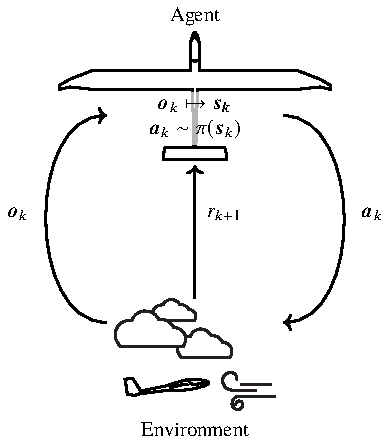
\includegraphics[width=0.5\textwidth]{src/pics/RLProblem.pdf}
	\caption{The Agent-Environment-System \cite{Notter2018}}
	\label{fig:agent_env_system} 
\end{figure}

\section{Model Based and Model Free Learning}

MDP solution methods can be divided into model-free and model-based methods. In model-based methods, the agent uses a model to predict the reaction of the environment to any of his actions. An environment model typically takes a state-action pair and returns the next state and next reward. If the environment is stochastic, there are multiple possible next states and rewards. A \textit{sample model} returns one of the possibilities, whereas a \textit{distribution model} returns some representation of all possible next states and rewards.

Regardless of the type, all models approximate what might happen to the agent in future time steps. Whether the experience gathered through a model is useful obviously depends on its quality. To distinguish experience from a model from real experience, the results from a model are referred to as \textit{simulated experience}\cite{SuttonBarto2018}. Figure \ref{fig:model-based-model-free} shows some popular Machine Learning algorithms and classifies them.

\section{Agent}

The agent in an MDP consists of at least one of the following parts.

\begin{itemize}
	\item Policy: \\
	A mapping from states to actions that tells the agent what to do (c.f. section \ref{sec:policy})
	\item Value Function: \\
	A mapping from states (or state-action pairs) to values (c.f. section \ref{sec:value-function})
	\item Model: \\
	A model of the environment that might be updated by the agent's experience
\end{itemize}

Most agents have a policy. They also can have a value function, like in actor-critic algorithms where the value function is used for bootstrapping. This means utilizing the Bellman Expectation Equation to estimate the return $G_t$ by doing a one step lookahead and use the sum of the immediate reward and the successor state value.

\begin{align}
\mathbb{E}[G_t|s_t=s] &= \mathbb{E}[R_{t+1} + \gamma G_{t+1}|s_t=s, a_t=a] \\
&=\mathbb{E}[R_{t+1}+ \gamma V(s_{t+1})|s_t=s, a_t=a]
\end{align}

Instead of sampling a complete episode, bootstrapping makes it possible to learn from incomplete episodes.

A model of the environment is - in principle - not required for successful training. It can however be used to gather simulated experience and therefore reduce training time on a real agent like a robot. Although imperfect, information from a model can be useful in such cases where training time is restricted which particularly holds true for robots flying outdoors.

\section{Return}

The return $G_t$ at a time step $t$ is the cumulative reward $r_t$ at each step from the state $s_t$ onwards until reaching a terminal state:

\begin{equation}
G_t = \sum_{k=0}^{T-t-1}\gamma^k r_{t+k+1}
\end{equation}

If $\gamma \in (0,1]$ is close to zero, immediate rewards are weighted stronger. If $\gamma$ is close to one, rewards in the distant future are weighted likewise, making decisions more far sighted. In infinite horizon problems where there is no terminal state, $\gamma$ must be less than one in order to avoid infinite returns. In finite horizon (i.e. episodic) MDPs, $\gamma$ is usually close to, or exactly one.

Each decision at a given state $s_t$ also affects what the next state $s_{t+1}$ is and therefore the next reward. More on the reward and what role it plays in Dynamic Programming is explained in section \ref{sec:reward}

\section{Policy}
\label{sec:policy}
In reinforcement learning problems, a policy is usually the part that represents the agent. It contains all the information needed to decide what action to choose in each state the agent visits. A policy is a mapping from states to actions.

\begin{equation}
\pi: \mathcal{S} \times \mathcal{A} \mapsto [0,1]
\end{equation} 

The policy is a probability distribution over actions given states and returns - for each state - the probability of taking an action $a_t$. If the policy is deterministic, only one $a_t$ out of $\mathcal{A}$ has a probability of one with all other actions assigend to probability zero. In any policy, the sum of all possible action-probabilities must be one.

\begin{equation}
\pi(a|s) = \mathbb{P}[a_t=a|s_t=s]
\end{equation}

This yields equations \ref{eq:transprobpi} and \ref{eq:rewardpi} for the state transition probability and the reward function under policy $\pi$. The reward function is explained in section \ref{sec:reward-function}.

\begin{equation}
\mathcal{P}^\pi(s,s')=\sum_a \pi(a|s)\mathcal{P}(s'|s,a)
\label{eq:transprobpi}
\end{equation}
\begin{equation}
\mathcal{R}^\pi(s) = \sum_a\pi(a|s)\mathcal{R}(s,a)
\label{eq:rewardpi}
\end{equation}

At each timestep, the agent receives a state observation $o_{t-1}$ from the environment, passes it to the policy and the policy returns an action $a_t$. This action is taken and the agent gets a new observation $o_t$ and a reward $r_t$. This process is repeated until the agent reaches a terminal state.

A policy can be implemented in many different ways. The simplest option is a table where each field contains the action for one state or - if the policy is stochastic - all possible actions and their respective probabilities. Other examples include linear combinations of the inputs and linear combinations of basis functions. The most popular way to implement a policy is - however - through an artificial neural network (ANN). More information about neural networks is given in chapter \ref{chapter3}.  

\section{Value Functions}
\label{sec:value-function}

Some RL-algorithms try to find a policy directly from experience. Others, like Q-learning, additionally utilize a so called value function. A value function maps from states or state-action pairs to their values. In this context, the value of a state or an action is a measure of how useful it is for the agent to visit the respective state or choosing the respective action. There are two types of value functions, state value functions and action value functions. The state value $V(s)$ is the expected total return from state $s_t$ onwards until the episode terminates. The action value also takes into account what the agent chooses to do in state $s_t$. It is the expected total return from state $s_t$ when choosing action $a_t$.

\begin{equation}
V(s) = \mathbb{E}[G_t|s_t=s]
\label{eq:state_value_fun}
\end{equation}

\begin{equation}
Q(a|s) = \mathbb{E}[G_t|s_t=s,a_t=a]
\label{eq:action_value_fun}
\end{equation}

In the following sections, the action space is regarded finite for simplicity.
The state value function \ref{eq:state_value_fun} can be expressed in terms of the action value function \ref{eq:action_value_fun}:

\begin{equation}
V_\pi(s) = \sum_{a}\pi(a|s)Q_\pi(s,a)
\label{eq:state_value_function_with_q}
\end{equation}

Similarly, the action value function can be expressed by means of the state value function:

\begin{equation}
Q_\pi(s,a)=\mathcal{R}(s,a)+\gamma \sum_{s'}\mathcal{P}(s'|s,a)V_\pi(s')
\label{eq:action_value_function_with_v}
\end{equation}

If an agent has found the optimal value function $V^*$ or $Q^*$ of an MDP, the optimal policy $\pi^*$ can be derived directly by acting greedily with respect to the value function at each state.

Like a policy, a value function may be implemented as a table, a linear combination of the input features, a combination of basis functions, or an artificial neural network.

\section{The Bellman Expectation Equation}

According to the Bellman Expectation Equation, every trajectory through the state space can be decomposed into two parts: the next step and the rest of the path. Equivalently, every state value can be split into the value of the next step and the successor state value.

The state value function \ref{eq:state_value_fun} can be written as a weighted sum of the action values, each multiplied with the probability to take the respective action according to the policy. Replacing $Q_\pi(s,a)$ in equation \ref{eq:state_value_function_with_q} with equation \ref{eq:action_value_function_with_v} yields equation \ref{eq:bellman_exp_eq_V_Q} which is known as the \textit{Bellman Expectation Equation}:
\begin{align}
V_\pi(s)&=\sum_a \pi(a|s)Q_\pi(s,a)\\ &= \sum_a \pi(a|s)\sum_r \sum_{s'} \mathcal{P}(s',r|s,a)[r+\gamma V_{\pi}(s')]
\label{eq:bellman_exp_eq_V_Q}
\end{align}

In a deterministic environment, equation \ref{eq:bellman_exp_eq_V_Q} becomes

\begin{equation}
V_\pi(s)= \sum_a \pi(a|s)[r+\gamma V_{\pi}(s')]
\label{eq:bellman_exp_eq_V_determinisic}
\end{equation}

The Bellman Expectation Equation can be used to update a state value by looking at the state values of its successor states and weighting them by the probabilities to reach each successor state (c.f. equations \ref{eq:bellman_exp_update_bootstrapped} and \ref{eq:bellman_exp_update_discrete}).

\section{The Bellman Optimality Equation}

Instead of a weighted sum of rewards and successor values, like in equation \ref{eq:bellman_exp_eq_V_Q}, one can take only the action that has the maximum action value. This yields the following equation:

\begin{align}
V_*(s)&=\max_{a \in \mathcal{A}(s)} Q_{\pi_*}(s,a) \label{eq:bellman_optimality_equation_v_with_q}\\
&=\max_{a}\mathbb{E}_{\pi_*}[G_t|s_t=s,a_t=a]\\
&=\max_{a}\mathbb{E}_{\pi_*}[R_{t+1} + \gamma G_{t+1}|s_t=s,a_t=a]\\
&=\max_{a}\mathbb{E}[R_{t+1} + \gamma V_*(s_{t+1})|s_t=s,a_t=a]\\
&=\max_{a}\sum_{s',r}\mathcal{P}(s',r|s,a)[r + \gamma V_*(s')]
\label{eq:bellman_optimality_equation_stochastic}
\end{align}

Again, if the environment is deterministic, equation \ref{eq:bellman_optimality_equation_stochastic} can be simplified:

\begin{equation}
V_*(s) = \max_a[r+\gamma V_*(s')]
\label{eq:bellman_optimality_equation_deterministic}
\end{equation}

All equations from \ref{eq:bellman_optimality_equation_v_with_q} to \ref{eq:bellman_optimality_equation_deterministic} are alternative ways to express the \textit{Bellman Optimality Equation}. It states that the value of a state under an optimal policy must equal the expected return for the best action in that state \cite{SuttonBarto2018}. Intuitively it is obvious that the optimal policy must pick the best action in each state. In Value Iteration, the \textit{Bellman Optimality Equation} is used as an update rule. See chapter \ref{subsection:VI} for more details.
% !TeX root = ../../../Main.tex
\chapter{Dynamic Programming}
\label{chapter3}

\begin{figure}[h]
	
\includegraphics[width=\textwidth]{src/pics/dummy.jpg}
	\caption{Classification of Machine Learning algorithms}
	\label{fig:model-based-model-free} 
\end{figure}

This thesis deals with Dynamic Programming for policy optimization. Markus Zuern very successfully applied Trust Region Policy Optimization (TRPO) to a 2D trajectory optimization problem\cite{Zuern2017}. In the same work, he compared Asynchronous Advantage Actor Critic (A3C) to TRPO. Both algorithms deal with the complete environment, i.e. the glider dynamics and the stochastic wind distribution, at the same time. Whereas the wind distribution is unknown a priori, the glider dynamics are well known. Therefore, a DP algorithm can be applied to any scenario with calm air. The resulting optimal policy $\pi^*_{\text{calm}}$ (todo: dies überall übernehmen) then can be used as a starting point for TRPO in scenarios with unknown wind conditions.

\begin{figure}[h]
	
\includegraphics[width=\textwidth]{src/pics/dummy.jpg}
	\caption{Figure 3.1 von Markus}
	\label{fig:RLmethods} 
\end{figure}

Dynamic programming is a general term, that is used for algorithms that solve a specific type of problem. Those problems can be decomposed into subproblems and solved by composing the solutions of those subproblems. If the subproblems are very similar, the solution of one subproblem can be used to calculate another one. In such cases, dynamic programming is applicable. In MDPs, these subproblems are similar in the sense that the Bellman Expectation Equation and the Bellman optimality equation hold true in all states, i.e. each state (and action) value is connected to its successor values by one of the Bellman Equations.

Also, the optimal action is found in all states the same way, as can be seen in section \ref{sec:PI}. If the algorithm is successful, the policy is optimal according to section \ref{sec:optimality}. Unlike with TRPO, optimization is not done through sampling complete trajectories, but by iterating the state-values and policy for each state independently. After one sweep over the state space, the value function and policy are updated and the process is repeated.\bigbreak

In theory, starting TRPO or A3C with a policy that is already optimal with respect to the scenario in calm air should accelerate training with updrafts because the information about how to behave in a situation with no wind is already "saved" in the policy.

\section{Approximate Dynamic Programming}

(hier noch einfügen, wie DP mit RL zusammenhängt)

\section{Reward Function}
\label{sec:reward-function}

As shown in Fig. \ref{fig:agent_env_system}, the agent interacts with his environment by, at each time step, picking an action $a_t$ and receiving an observation $o_t$ and a reward $r_t$. In RL, the reward function is the only means to give the agent information about what he should or should not do.

The reward function in this work is as follows:

\begin{equation}
\mathcal{R}(s,a): \mathcal{S} \mapsto \mathbb{R}: r_t =
\begin{cases}
-\Delta t & \text{if } s_{t+1} \neq s_{T+}\\
-\Delta t + \frac{d}{10} & \text{if } s_{t+1} = s_{T+}
\end{cases}
\label{eq:reward_function}
\end{equation}

(todo: abbildung dazu?)

where $s_{T+}$ is a terminal state that is also a target state. There are terminal states $s_{T-}$ where the agent is not meant to go. These terminal states are those where the agent touches the ground before reaching his target range. If the agent reaches his goal, he receives a final reward $r_T$ according to the second line of Eq. \ref{eq:reward_function}. 

It is possible to penalize undesired behavior of the agent by defining a large negative reward if, for example, the agent touches the ground before reaching the target distance or flies too far in the wrong direction. This is, however, not necessary, if the final reward is sufficiently high. If the agent has to cover a distance of 500 m, he receives a final reward of +50. with a mean ground speed of about $15-20\frac{\text{m}}{\text{s}}$, covering 500 m takes between 25 and 33.3 s. If the agent gets $-1$ reward per second it takes him to reach 500 m, the expected return from a state far away from the goal can still get up to about $33.3\cdot (-1) +50=16.7$. This would not work if the final reward was only $+\frac{\text{d}}{20}$. The important thing here is, that reaching a target state must always yield a higher return than ending an episode on the ground from any state $s \in \mathcal{S}$.


\section{The Principle of Optimality}
\label{sec:optimality}

According to Bellman's principle of optimality, the solution of some optimization problems can be put together from the solution of subproblems. This is the basis for all dynamic programming algorithms. If an agent chooses the optimal action in a state $s_t$ and all states it visits afterwards ($s_k$, $k=t+1, t+2, ...,T$) , the resulting trajectory is the optimal one from $s_t$ to the terminal state $s_T$.

The term \textit{principle of optimality} was first used by Richard E. Bellman in 1954 \cite{Bellman1954}. He proved that various optimization problems could be solved efficiently by making use of the principle of optimality instead of traditional optimal control theory. In his book \textit{Applied Dynamic Programming}, Bellman covered numerous examples of optimal control problems and shows how they can be solved by Dynamic Programming \cite{Bellman1962}.

\section{Types of Dynamic Programming Algorithms}

\subsection{Policy Evaluation}
\label{subsection:policy_evaluation}

In Policy Evaluation, the goal is to find an approximation of the value function $V_\pi$ that corresponds to a given policy $\pi$. The value of a state is defined as the expected total return from that state onwards until the episode terminates. Obviously, the expectation in equation \ref{eq:bellman_exp} depends on the actions that are taken at each step and therefore on the policy that is evaluated. The state value that corresponds to a specific policy $\pi$ is denoted by $V_\pi(s)$.

\begin{align}
V_\pi(s_t)&=\mathbb{E}[G_t|s_t=s]\\ &= \mathbb{E}\left[ \sum_{k=0}^{T-t-1}\gamma^k r_{t+k+1}|s_t=s\right] \\
&=\mathbb{E}[r_{t+1}+\gamma^1 r_{t+2}+\gamma^2 r_{t+3}+\gamma^3 r_{t+4}+...+\gamma^{T-t-1}r_T|s_t=s]
\label{eq:bellman_exp}
\end{align}

With a stochastic discrete policy, equation \ref{eq:bellman_exp} becomes

\begin{equation}
V_\pi(s_t)=\sum_{a}\pi(a|s)(\mathcal{R}(s,a)+\gamma V_\pi(s'))
\label{eq:bellman_exp_discrete_policy}
\end{equation}

Recall the definition of a state value $V(s) = \mathbb{E}[G_t|s_t=s]$ from Eq. \ref{eq:state_value_fun}. This equation can be used as a mapping to update the value of $s_t$ with the expected return according to the current policy.

\begin{equation}
V_\pi(s_t) \mathrel{\reflectbox{\ensuremath{\mapsto}}} \mathbb{E}[ \sum_{k=0}^{T-t-1}\gamma^k r_{t+k+1}|s_t=s]
\label{eq:bellman_exp_update}
\end{equation}

In Eq. \ref{eq:bellman_exp}, all terms expect the first one can be replaced by the expected return from $s_{t+1}$ onwards:

\begin{align}
V_\pi(s_t) \mathrel{\reflectbox{\ensuremath{\mapsto}}} 
&\;\mathbb{E}[r_{t+1}+\gamma G_{t+1}|s_t=s]\\
=&\;r_{t+1}+\gamma V_\pi(s_{t+1})
\label{eq:bellman_exp_update_bootstrapped}
\end{align}

With a discrete stochastic policy, equation \ref{eq:bellman_exp_update_bootstrapped} becomes


\begin{equation}
V_{\pi}(s_t) \mathrel{\reflectbox{\ensuremath{\mapsto}}} \sum_{a}\pi(a|s)(r_t+\gamma V_\pi(s'))
\label{eq:bellman_exp_update_discrete}
\end{equation}

In a state space with a finite set of states $\mathcal{S}$, writing down Eq. \ref{eq:bellman_exp_update_discrete} for each state results in a system of $|\mathcal{S}|$ linear equations that can be solved for $V(s)$. If the number of states is very large, this is not very efficient. 

Instead, \ref{eq:bellman_exp} is usually solved iteratively. The simplest way is to perform a one step lookahead from each state to get $r_t$ and $V(s_{t+t})$ from the current estimate of the state value function. Once all values are calculated, the values of all states are updated simultaneously \footnote{There are variants of Policy Iteration, where the updates are performed asynchronously. This means that, for example, all neighbors of a terminal state are updated first. After that, the states, that lie next to these states, are updated, and so on. They usually converge faster, but at the expense of implementation complexity.}. Unlike other RL-algorithms, the state values are not updated along a trajectory. Instead, each state is updated independently.

Each set of state values approximates the true value function of the problem better than the previous set of estimates. Every state value converges to the true state value under the given policy. It is not efficient to wait until the values have fully converged, i.e. the true value function $V_\pi$ is reached. Instead the process is repeated until the maximum absolute change in values lies beneath a certain threshold $\epsilon_V$. This maximum absolute change can be expressed by the supremum-norm $||(\cdot)||_\infty$ (c.f. section \ref{sec:contraction_mappings}). Algorithm \ref{algo:pe} shows a possible implementation of iterative policy evaluation.

\begin{equation}
||V_{k}-V_{k-1}||_\infty<\epsilon_V
\label{eq:pe_stopping_criterion}
\end{equation}

\begin{algorithm}[hbt]

	\begin{algorithmic}[0] % 1 to show code line numbers
		
		\Function{Policy Evaluation}{}
			\State Initialize $V(s) = 0 \; \forall \; s \in \mathcal{S}$ and load policy $\pi$.
			\While {true}
				\ForAll{$s \in \mathcal{S}$}
					\State $V_{\pi,new}(s) \mathrel{\reflectbox{\ensuremath{\mapsto}}} r+\gamma V_ {\pi,old}(s')$
				\EndFor
				\State update value function
				\If {$||V_{new}-V_{old}||_\infty \leq \epsilon_V$}
					\State break
				\EndIf
			\EndWhile
		\EndFunction
	\end{algorithmic}
	\caption{Iterative policy evaluation}
	\label{algo:pe}
\end{algorithm}

\subsection{Policy Iteration}
\label{sec:PI}
Policy iteration is an iterative way to calculate an estimate of the optimal policy of an MDP. Starting with an arbitrary policy and value function, one iteration of policy evaluation is performed to get an estimate of $V_\pi$. After that, after that, the policy is replaced by the greedy policy w.r.t. to the new value function estimate $V_\pi$. This alternating process of Policy Evaluation and Policy Improvement is repeated until the policy is satisfactory.

\begin{equation}
a_{\text{greedy}}(s_t) = \underset{a}{\text{argmax}}[Q(s_t,a_t)]
\end{equation}

For a deterministic, greedy policy $\pi_{\text{greedy}}$, this yields:

\begin{align}
\pi(a_{\text{greedy}}|s_t)&=\mathbb{P}[a_t=a_{\text{greedy}}(s_t)|s_t] \\ &=1
\end{align}

and for a stochastic policy $\pi$:

\begin{equation}
\mathbb{E}[\pi(a_t | s_t)] \mathrel{\reflectbox{\ensuremath{\mapsto}}} a_{\text{greedy}}
\end{equation}

As mentioned in subsection \ref{subsection:policy_evaluation}, each policy evaluation step usually ends if the maximum difference between two subsequent values of the same state are sufficiently close.

There is a version of Policy Iteration where only one value update is done before updating the policy. This algorithm is called Optimistic Policy Iteration (OPI). Although the first estimate of the value function is only a rough approximation, OPI also converges to the optimal value function and policy. The following diagram illustrates the policy iteration scheme.

\begin{equation*}
\pi_0 \overset{evaluate}{\longrightarrow} V_1 \overset{improve}{\longrightarrow} \pi_1 \overset{evaluate}{\longrightarrow} V_2 \overset{improve}{\longrightarrow} \pi_2 \overset{evaluate}{\longrightarrow} ... \overset{evaluate}{\longrightarrow} V_* \overset{improve}{\longrightarrow} \pi_*
\label{eq:pi_scheme}
\end{equation*}

Another way to picture Policy Iteration is shown in figure \ref{fig:PI_triangle}. Every PI-step brings the Value Function $V(s)$ closer to $V_*(s)$ and the policy $\pi$ closer to $\pi_*$.

\begin{figure}[h]
	
\includegraphics[width=\textwidth]{src/pics/dummy.jpg}
	\caption{The policy iteration algorithm}
	\label{fig:PI_triangle} 
\end{figure}

The performance of both algorithms on the trajectory optimization problem is compared in chapter \ref{chapter6}. \bigbreak

In a discrete MDP, there is a finite number of states and actions. At each state $s \in \mathcal{S}$, the agent can choose the action $a$ from a set $\mathcal{A}$ of possible actions. In such a scenario, there exist $|\mathcal{A}|^{|\mathcal{S}|}$ different policies. It therefore takes $|\mathcal{A}|^{|\mathcal{S}|}$ iterations to find the optimal policy assuming no policy occurs twice. If that was the case, this policy would have to occur in two subsequent iterations and therefore be the fixed point $\pi_*$ of the policy sequence generated by PI.

As the results in chapter \ref{chapter6} show, PI and VI converge much faster in practice than the upper bound $|\mathcal{A}|^{|\mathcal{S}|}$ may suggest. Algorithm \ref{algo:gpi} shows one way to implement generalized policy iteration. The pseudocode for optimistic policy iteration can be found in algorithm \ref{algo:opi} in appendix \ref{appendix_D}.

\begin{algorithm}[hbt]
	\begin{algorithmic}[0] % 1 to show code line numbers
		\Function{Generalized Policy Iteration}{}
			\State Initialize $V(s) = 0 \; \forall \; s \in \mathcal{S}$
			\State Load arbitrary initial policy $\pi_0$.
			\State Initialize $m$,\;$\epsilon_V$
			\While {true}			
			\Function{Policy Evaluation}{}
				\While {true}
				\ForAll{$s \in \mathcal{S}$}
					\State $V_{\pi,new}(s) \mathrel{\reflectbox{\ensuremath{\mapsto}}} r+\gamma V_ {\pi,old}(s')$
				\EndFor
				\State update value function
				\If {$||V_{new}-V_{old}||_\infty \leq \epsilon_V$}
					\State break
				\EndIf
				\EndWhile
			\EndFunction
			\Function{Policy Improvement}{}
				\ForAll{$s \in \mathcal{S}$}
					\State sample $m$ actions $a_n(s)$
					\ForAll {$a_n$}
						\State $Q(s,a_n) = r + \gamma V(s')$
					\EndFor
					\State $a_{greedy}(s)=\underset{a_n}{\text{argmax}}[Q(s,a_n)]$
				\EndFor
			\EndFunction
			\State
			\State train policy on $a_{greedy,new}$ to obtain $\pi_{new}$
			\If {$||a_{greedy,new}-a_{greedy,old}||_\infty = 0$}
				\State break
			\EndIf

			\EndWhile
			\State
		\EndFunction
	\end{algorithmic}
	\caption{Generalized policy iteration}
	\label{algo:gpi}
\end{algorithm}

\subsection{Value Iteration}
\label{subsection:VI}
Value iteration is similar to policy iteration, but instead of calculating a new policy at each iteration step, the state values $V(s)$ are directly updated with the maximum possible successor value that is achievable starting from $s$. This yields a sequence of value functions, each one being a better estimate of $V_*$ than its predecessor. Each of the intermediate value functions is abstract in so far as there does not have to exist an explicit policy corresponding to it (c.f. \cite[lecture~3]{Silver2015}). In a possibly discounted MDP with a deterministic environment, the update rule for each state value can be seen in equation \ref{eq:value_iteration_update}.

\begin{equation}
V(s_t) \mathrel{\reflectbox{\ensuremath{\mapsto}}} 
\underset{a}{\text{max}}[r_{t+1}+\gamma V(s_{t+1})|s_t=s]
\label{eq:value_iteration_update}
\end{equation}

In principle, this is equivalent to synchronous OPI, where after one state value update at each state, the policy is replaced by the greedy policy with respect to the new value function. The only difference is, that value iteration does not output an intermediate policy at each iteration. Instead, it only iterates value functions. 

\begin{equation*}
V_1 \longrightarrow V_2 \longrightarrow V_3 \longrightarrow ... \longrightarrow  V_*
\label{eq:vi_scheme}
\end{equation*}

In practice, a stopping criterion is introduced to limit calculation time. In this work, iteration is stopped if $||V_{k}-V_{k-1}||_\infty<\epsilon_V$, identical to equation \ref{eq:pe_stopping_criterion}. The last iterate $V_n$ is considered an approximation of $V_*$. If $V_n$ is close enough to the true optimal value function $V_*$, the (approximately) optimal policy can be calculated in the end by acting greedily with respect to $V_n$. Recall that, if Value Iteration is stopped too early, there might not even be a real policy that corresponds to the last value function iterate $V_n$ \cite[lecture~3]{Silver2015}. A possible implementation of value iteration is shown in algorithm \ref{algo:vi}.

\begin{algorithm}[hbt]
	\begin{algorithmic}[0] % 1 to show code line numbers
		\Function{Value Iteration}{}
			\State Initialize $V(s) = 0 \; \forall \; s \in \mathcal{S}$
			\State Initialize $m$,\;$\epsilon_V$
			\While {true}	
				\ForAll {$s \in \mathcal{S}$}
					\State sample $m$ actions $a_n(s)$
					\ForAll {$a_n$}
						\State $Q(s,a_n) = r + \gamma V(s')$
					\EndFor		
					\State $V_{new}(s)=\underset{a_n}{\text{max}}[Q(s,a_n)]$
				\EndFor
				\If {$||V_{new}-V_{old}||_\infty \leq \epsilon_V$}
					\State break
				\EndIf
			\EndWhile
			\Function{Policy Improvement}{}
				\ForAll{$s \in \mathcal{S}$}
					\State sample $m$ actions $a_n(s)$
					\ForAll {$a_n$}
						\State $Q(s,a_n) = r + \gamma V(s')$
					\EndFor
					\State $a_{greedy}(s)=\underset{a_n}{\text{argmax}}[Q(s,a_n)]$
				\EndFor
			\EndFunction
			\State train policy on the latest $a_{greedy,new}$ to obtain an estimate of $\pi_*$
		\EndFunction
	\end{algorithmic}	
	\caption{Value iteration}
	\label{algo:vi}
\end{algorithm}

\section{The Contraction Mapping Theorem}
\label{sec:contraction_mappings}
A contraction mapping $f: M \to M$ on a metric space $M$ has the following property:
\begin{equation}
|f(x_1)-f(x_2)| \leq \gamma |x_1-x_2|
\end{equation}

with $x_1,x_2 \in M$ and $\gamma \in [0,1)$. In this context,  $|(\cdot)|$ denotes an arbitrary metric on $M$.

The term contraction reflects the fact that, graphically speaking, a contraction mapping reduces the distance between $x_1$ and $x_2$.

\subsubsection{Discounted MDPs}

Policy Evaluation in discounted MDPs is a contraction mapping. This result can be obtained in few steps. The mapping in equation \ref{eq:bellman_exp_update_discrete} and \ref{eq:bellman_operator_discounted} is known as the \textit{Bellman Operator}. It maps from a state value function to a state value function. If the Bellman Operator is applied multiple times, this can be expressed by $T^n(v)$.

\begin{equation}
T_\pi(v(s'))=\mathcal{R}_\pi+\gamma \mathcal{P}_\pi v(s')
\label{eq:bellman_operator_discounted}
\end{equation}

If the Bellman Operator is applied to two state value functions $V_1(s)$ and $V_2(s)$, it reduces the distance between the two in value function space. This distance can be expressed by the supremum norm, which is defined as follows:

\begin{equation}
||V||_\infty = \max_{s \in \mathcal{S}} |V(s)|
\end{equation}

The supremum norm of $V_1 - V_2$ is therefore

\begin{equation}
||V_1(s) - V_2(s)||_\infty = \max_{s \in \mathcal{S}} |V_1(s)-V_2(s)|
\end{equation}

which is the biggest absolute difference of values of the same state in the state space. If the Bellman Operator is applied to both $V_1$ and $V_2$, the contraction property proof is straightforward. For simplicity, the arguments of $V_1(s)$ and $V_2(s)$ are omitted in the following equations.
\begin{align}
||T_\pi(V_1)-T_\pi(V_2)||_\infty &= ||(\mathcal{R}_\pi+\gamma \mathcal{P}_\pi V_1)-(\mathcal{R}_\pi+\gamma \mathcal{P}_\pi V_2)||_\infty \label{eq:4.15}\\
&=||\gamma\; \mathcal{P}_\pi\;(V_1 - V_2)||_\infty \label{eq:4.16}\\
&\leq ||\gamma \mathcal{P}_\pi ||V_1 - V_2||_\infty ||_\infty \label{eq:4.17} \\
&\leq ||\gamma ||V_1 - V_2||_\infty ||_\infty \label{eq:4.18}\\
&=\gamma ||V_1 - V_2||_\infty \label{eq:4.19}
\end{align} 

Whenever $s'$ happens to be the state where $V_1$ and $V_2$ differ the most, equality holds in line \ref{eq:4.17}. If not, applying the supremum norm to $V_1(s')-V_2(s')$ increases the value of the expression. $\mathcal{P}_\pi$ must always be smaller than or equal to one. Similar to line \ref{eq:4.17}, equality in line \ref{eq:4.18} holds only if $\mathcal{P}_\pi=1$. Replacing $\mathcal{P}_\pi$ by one in line \ref{eq:4.17} yields line \ref{eq:4.18}. The left side of line \ref{eq:4.15} must thus be less than line \ref{eq:4.19} which proves the contraction property of the Bellman Operator in discounted MDPs.

\subsubsection{Undiscounted MDPs}

An MDP, where the discount factor $\gamma$ is one, is called an undiscounted MDP. In such an MDP, the Bellman Operator looks like in equation \ref{eq:bellman_undiscounted}.

\begin{equation}
T_\pi(v(s))=\mathcal{R}_\pi + \mathcal{P}_\pi V(s')
\label{eq:bellman_undiscounted}
\end{equation}

If $\gamma$ is one, the above proof of the contraction property does not hold anymore. It can however be proven, that the Bellman Operator still contracts. In the undiscounted case, this takes more than one step. Equation \ref{eq:n-step-contraction} shows the n-step contraction property. For simplicity, the index $\pi$ and the argument $s$ are omitted.

\begin{equation}
||T^{(n)}(V_1)-T^{(n)}(V_2)||_\infty \leq ||V_1-V_2||_\infty
\label{eq:n-step-contraction}
\end{equation}

Equation \ref{eq:n-step-contraction} means, that applying the Bellman Operator n times to two value functions brings them closer together in value function space. As a result, the Bellman Operator also leads to $V_1 \approx V_2$ eventually also in undiscounted MDPs.

A proof, that policy iteration and value iteration also converge in undiscounted MDPs, can be found in \cite{},\cite{} and \cite{}.


% !TeX root = ../../../Main.tex

\chapter{Function Approximation}
\label{chapter4}

A common problem in engineering is developing a model from measurement data. Such a model makes it possible to generalize from the given data to new data, for which a real measurement does not exist. The process of developing a model is often combined with function approximation. The goal here is to find a mapping as a linear combination of elements, which constitute a basis from functions, that approximates a given behavior, also called a target function, as close as possible.

Mathematically, function approximation is the process of finding a mapping from inputs $x$ to outputs $y$. Usually, a set $\mathcal{X}=\{x_{fit,1},x_{fit,2},...\}$ of inputs and a set $\mathcal{Y}=\{y_{fit,1},y_{fit,2},...\}$ corresponding desired outputs is given and the goal is to find a function that returns a value close to $y_{fit,i}$ for each $x_{fit,i}$.

There are two types of function approximation. In some cases, knowledge about the specific problem can help to find suitable base functions. If, for example, a mapping is known to be linear ($y=a_0 + a_1 x$), the function approximation process degenerates to finding the two coefficients $a_0$ and $a_1$. The same applies to quadratic, trigonometric or exponential target functions or linear combinations of them. If, however, the target function is not known, function approximation is more elaborate. One can try multiple target functions or combine them in order to find one, that fits best, or use a \textit{universal function approximator} like an artificial neural network. 

\section{Tables}

The simplest way to express a discrete mapping is by a table where each input/output pair is represented by a cell of the table. The number of inputs and corresponding outputs in a table is inherently finite. The set of states and actions in a continuous MDP is however infinite, so the policy and value functions must also be continuous. If a discrete mapping like a table is used as a representation of a policy or value function in a continuous MDP, it will, at some point, be confronted with unknown inputs. The inability to deal with unknown inputs is a big disadvantage of tables. There are, however, ways to overcome this weakness.

\subsubsection{Nearest Neighbor}

The most straightforward way to obtain an output for an unknown input is to look for the table entry that is closest to the unknown input. This yields a piecewise constant mapping from inputs to outputs and enables the table to generalize. Whether this suffices as an approximation for a continuous mapping $f$ heavily depends on the properties of $f$ . If there are large differences between the output of two subsequent inputs, the error can be very high.

\subsubsection{Linear Interpolation}

Another way to obtain outputs for unknown inputs is to interpolate linearly. In a first step, the two nearest known inputs $x_0$ and $x_1$ and their respective outputs $y_0$ and $y_1$ are looked up (note that $x_0 \leq x \leq x_1$ in this case). In the second step, the output is calculated by the following formula:

\begin{equation}
y_{interp} = y_0 \cdot (1-\gamma) + y_1 \cdot \gamma
\end{equation}

where $\gamma = \frac{x - x_0}{x_1 - x_0}$.

One advantage of linear interpolation of table values is that the output is at least continuous, though not differentiable at the known input points.

\section{Artificial Neural Networks}

The structure of artificial neural networks resembles the structure of a human brain according to the current state of research \cite[Chapter~1.1]{Kriesel2007NeuralNetworks}. The human brain consists of a very high number of neurons, each receiving signals from other neurons, processing them and itself sending a signal to other neurons if certain conditions are met. Each neuron is very simple, it is the high number of them and the fact that they all work in parallel that makes the human brain so powerful. 

\begin{figure}[h]
	\centering
	\tikzsetnextfilename{neuron}
	\label{tikz:neuron}	
	\begin{tikzpicture}
	
	\pgfplotsset{
		width=0.8\textwidth,
		height=0.9\textwidth, 
		xmajorgrids, 
		ymajorgrids, 
		enlarge x limits=false,
		scaled x ticks = false,
		x tick label style={/pgf/number format/.cd, fixed, set thousands separator={}},
		scaled y ticks = false,
		yticklabel style={/pgf/number format/.cd, fixed, set thousands separator={}},
		xmin=0, xmax=6,
		legend pos=north west,
		legend cell align=left
	}
	\node[circle, draw=black, fill=white] at (0,0) {$\sum$};
	\node at (-3.6,3) {Inputs};
	\node at (-2,3) {Weights};
	\node[text width=4cm,align=center] at (2,1) {Activation \\ function};
	\node[align=center] at (4,1) {Output};
	\node at (-3.6,2) {$c_1$};
	\node at (-3.6,0) {$c_2$};
	\node at (-3.6,-2) {$c_3$};
	\node at (-2,2) {$w_1$};
	\node at (-2,0) {$w_2$};
	\node at (-2,-2) {$w_3$};
	\node[text width=1cm,align=center] at (0,2.8) {Bias \\ $b$};
	\node[draw=black] at (2,0) {$h$};
	\node at (4,0) {$z$};
	\draw[->] (-1.8,1.8) -- (-0.35,0.35);
	\draw[->] (-1.75,0) --  (-0.5,0);
	\draw[->] (-1.8,-1.8) -- (-0.35,-0.35);
	\draw[->] (0,2.2) -- (0,0.5);
	\draw[->] (0.5,0) -- node [above] {$a$} (1.75,0);
	\draw[->] (-3.3,0) -- +(1,0);
	\draw[->] (-3.3,2) -- +(1,0);	
	\draw[->] (-3.3,-2) -- +(1,0);
	\draw[->] (2.25,0) -- +(1.5,0);
	
	\end{tikzpicture}
	\caption{A neuron in an artificial neural network}
\end{figure}

A neuron in an artificial neural network looks like what is depicted by Fig. \ref{tikz:neuron}. It takes an arbitrary number of inputs $c_i$, multiplies each input by the corresponding input weight $w_i$, adds a bias and applies to the result $a$ a nonlinear function, the so called activation function $h$, yielding $z$, the neuron output. This output can either serve as an input to another neuron or as the network output. Multiple activation functions are common, most of which are somewhat s-shaped. These activation functions map the set of real numbers to the range between $-1$ and $1$ or sometimes between $0$ and $1$, limiting the neuron output and therefore its influence on the output of the ANN network. Examples include the step function, ($z=1$ if $x \geq x_0$, $z=0$ otherwise), the rectifier nonlinearity ($h(x)=\max(0,x)$), the sigmoid function ($h(x)=1/(1+e^{-x})$) and the tanh-activation function ($h(x)=\tanh(x)=\frac{e^x-e^{-x}}{e^x+e^{-x}}$).
Nonlinearity is essential here, because if linear activation functions are used, each neuron output is a linear function of its inputs. Any combination of linear mappings is itself linear. So if a deep neural network has only linear activation functions, the ANN output is always a linear function of the inputs, regardless of the number of hidden layers. Therefore, a deep neural network, where all activation functions are linear, can be replaced with a network, that has only one hidden layer (or something that is even simpler). The computational expense of dealing with a deep ANN is - however - very high compared to one with a single hidden layer. A deep ANN with only linear activation functions therefore does not make sense.

\begin{figure}[h]
	
\includegraphics[width=\textwidth]{src/pics/dummy.jpg}
	\caption{Activation functions \cite{Zuern2017}}
	\label{fig:activation_functions} 
\end{figure}

In an artificial neural network, the neurons are arranged in layers. The ANNs in this work are all fully connected feed forward networks, also known as Multi Layer Perceptrons (MLPs)\nomenclature[A]{MLP}{multi layer perceptron}. Each neuron in a given layer $k$ gets an input from each neuron in the previous layer $k-1$ and outputs a signal to each neuron in the next layer $k+1$ (c.f. Fig. \ref{tikz:neuron}).

\begin{figure}[h]
	\centering
	\tikzsetnextfilename{MLP}	
	\begin{tikzpicture}
	
		\pgfplotsset{
			width=0.8\textwidth,
			height=0.9\textwidth, 
			xmajorgrids, 
			ymajorgrids, 
			enlarge x limits=false,
			scaled x ticks = false,
			x tick label style={/pgf/number format/.cd, fixed, set thousands separator={}},
			scaled y ticks = false,
			yticklabel style={/pgf/number format/.cd, fixed, set thousands separator={}},
			xmin=0, xmax=6,
			legend pos=north west,
			legend cell align=left
		}
		
		
		\fill[black] (2,-2) circle (4pt) ;
		\fill[black] (2,-0) circle (4pt) ;
		\fill[black] (5,-3) circle (4pt) ;
		\fill[black] (5,-2) circle (4pt) ;
		\fill[black] (5,-1) circle (4pt) ;
		\fill[black] (5,0) circle (4pt) ;
		\fill[black] (5,1) circle (4pt) ;
		\fill[black] (8,-3) circle (4pt) ;
		\fill[black] (8,-2) circle (4pt) ;
		\fill[black] (8,-1) circle (4pt) ;
		\fill[black] (8,0) circle (4pt) ;
		\fill[black] (8,1) circle (4pt) ;
		\fill[black] (11,-2) circle (4pt) ;
		\fill[black] (11,0) circle (4pt);
	
	  	\foreach \a in {-2,0}
	  		\foreach \b in {-3,-2,-1,0,1}
				\draw (2,\a) -- (5,\b);
		
	  	\foreach \c in {-3,-2,-1,0,1}
			\foreach \d in {-3,-2,-1,0,1}
				\draw (5,\c) -- (8,\d);
				
		\foreach \e in {-3,-2,-1,0,1}
			\foreach \f in {-2,0}
				\draw (8,\e) -- (11,\f);
		
		\node[text width= 3cm,align=center] at (2,2) {input layer};
		\node[text width= 3cm,align=center] at (5,2) {hidden layer 1 \\ 64 neurons};
		\node[text width= 3cm,align=center] at (8,2) {hidden layer 2 \\ 64 neurons};
		\node[text width= 3cm,align=center] at (11,2) {output layer};
	
		\node[text width= 3cm,align=center] at (2,-4) {linear};
		\node[text width= 3cm,align=center] at (5,-4) {tanh};
		\node[text width= 3cm,align=center] at (8,-4) {tanh};
		\node[text width= 3cm,align=center] at (11,-4) {linear};
		
		\node at (1,-1) {s};
		\node at (12.5,0) {$\mu$};
		\node at (12.5,-2) {$\sigma$};
		
		\draw[->] (11,0) -- +(1,0);
		\draw[->] (11,-2) -- + (1,0);
		
		\draw[decorate,decoration=brace] (1.6,-2.2) -- (1.6,0.2);
		
	\end{tikzpicture}
	\label{tikz:MLP}
	\caption{The MLP used for the policy}
\end{figure}

If a policy or value function is represented by an artificial neural network (ANN\nomenclature[A]{ANN}{Artificial Neural Network}), the output for each state (or state-action-pair) is determined by the weights and biases of the network and the activation functions. As the latter are usually given or predetermined (and not trained), only the weights and biases are usually regarded as parameters. One set of weights and biases forms the \textit{parameter vector} $\theta$ of the neural network. If, for example, a stochastic policy is parametrized by $\theta$ and represented by a neural net with $k$ layers, the notation is as follows:

\begin{equation}
\pi_\theta(a|s)=\mathbb{P}[a|s,\theta]
\end{equation}

with

\begin{equation}
\theta = \{\boldsymbol{W}^{(1)},\boldsymbol{b}^{(1)},\boldsymbol{W}^{(2)},\boldsymbol{b}^{(2)}, ...,
\boldsymbol{W}^{(k)},\boldsymbol{b}^{(k)}\}
\label{eq:theta}
\end{equation}

The policy ANN does not necessarily need to output the action directly. Instead, most RL-related policies are stochastic, i.e. the neural net outputs the mean and standard deviation of a normal distribution:

\begin{equation}
\pi_\theta(\mu_\theta,\sigma_\theta|s)=\frac{1}{\sqrt{2\pi}\sigma_\theta}e^{-\frac{(a-\mu_\theta)^2}{2\sigma_\theta^2}}
\end{equation}

The action $a$ is then drawn from $\mathcal{N}(\mu_\theta(s),\sigma^2_\theta(s))$. 
In this work, the policy is represented with a neural network that has two outputs, the mean and standard deviation. Dynamic Programming is used only to find the optimal mean values. The standard deviation is set to 0.5. This serves as an intial solution for the policy net to be trained by an RL method.

\subsection*{Input Standardization}

All training algorithms that are used in this work rely on the partial derivative of a loss function with respect to the network weights and biases. As can be seen in Eq. \ref{eq:gd_update} and the following equations, they perform a step in (an approximation of) the current gradient direction. This gradient heavily depends on the network inputs. If some of the inputs have much larger values than the rest, this can result in some weights being updated faster than others, which is not desirable. Therefore, the inputs to a neural network should have the same scale. In this work, the inputs are scaled to a normal distribution with $\mu = 0$ and $\sigma = 1$:

\begin{equation}
\hat{x} = \frac{x - \mu}{\sigma}
\end{equation}

The specific values for $\mu$ and $\sigma$ for each of the scenarios are presented in table \ref{tab:glider_data}.

\subsection*{Action Scaling}

In an artificial neural network, every neuron can output a value between -1 and 1. Therefore, the output of a neural network is limited by the number of neurons in the last hidden layer. Obtaining a large output requires a lot of neurons. On the other hand, lots of neurons favor overfitting and increase training time. If the desired outputs are too small, then so are the neuron outputs. The $\text{tanh}(\cdot)$ activation function that is used for the policy is approximately linear in this area. Therefore the whole network behaves almost linearly if it is trained to output values close to zero and linear behavior can also be obtained without any hidden layers. The most important advantage of deep neural networks is however their ability to represent highly nonlinear behavior.

Both problems can be avoided if outputs lie between -1 and 1. This way, it is unlikely that any of the activation functions reach their saturation limit, nor is the network restricted to linear behavior. Therefore, the neural network is usually trained to output values between -1 and 1 and these values are then scaled to the desired magnitude by multiplying them with a scaling factor. Another way to mitigate this problem is choosing activation functions that are also nonlinear if the input and/or output is close to zero.

\subsection*{Weight initialization}

Training an artificial neural network is an iterative process. Therefore it requires initial values for the weights and biases. As training a neural network through supervised learning comes down to solving an optimization problem iteratively, training success highly depends on the initial weights.

The two most popular ways to initialize neural network weights are the Glorot uniform initialization and the glorot normal distribution. According to the glorot uniform initialization, the weights in one layer must be distributed uniformly within $\pm \sqrt{\frac{6}{n_{in}+n_{out}}}$ where $n_{in}$ and $n_{out}$ are the numbers of neurons in the prior and current layer, respectively.

The Glorot normal initialization states that the weights must be initialized according to a normal distribution with zero mean and a variance of $\sigma = \sqrt{\frac{2}{n_{in}+n_{out}}}$.

In this work, all neural networks are initialized according to the Glorot uniform distribution. 

\section{Supervised Learning}
All machine learning algorithms can be divided into two categories: supervised learning and unsupervised learning. In supervised learning, the agent is given the desired action for each state explicitly, so it knows what it is supposed to do. In unsupervised learning, however, the agent does not know what the best action is, so it has to find out itself. One way of doing that is from moving in the state space and learning from experience, for example by applying a reinforcement learning algorithm.

In the supervised learning case, training is done via minimizing a loss function that depends on the desired action and the actual action taken by the agent. A common loss-function is the mean squared error (MSE)\nomenclature[A]{MSE}{mean squared error} \nomenclature[L]{$\bar{e}$}{mean error}:

\begin{equation}
\bar{e} = \frac{1}{N}\;\sum_{n=1}^{N}{e}_{n} =  \frac{1}{N}\;\sum_{n=1}^{N}[\frac{1}{2}\;(a_n(s)-a_{fit,n})^2]
\label{lossfun}
\end{equation}

The goal of supervised learning is to minimize the difference between $a_{n,fit}$ and $a_n(s)$ in each state. If $a_n(s)$ is the output of a function approximator, minimizing $L_{MSE}$ is equivalent to fitting the function approximator to the desired outputs.

One advantage of the application of a loss function is that numerous iterative optimization algorithms have been developed to solve such a problem.

\section{Optimization Techniques}

As mentioned before, supervised learning is usually done by defining a loss function that depends on the network weights and biases and finding a local or global minimum numerically.

In this work, the ADAM algorithm is used for training the policy to output the desired action at each point in the state space. As most optimization algorithms, ADAM is gradient-based. Therefore, some insight into the general ideas behind gradient based numeric optimization is useful for understanding ADAM. Sections \ref{sec:grad_desc} and \ref{sec:sgd} explain briefly how gradient based optimization works in general. In section \ref{sec:adam}, ADAM is described and explained.

All presented algorithms produce a series of points in the space that the network weights and biases establish. The point at the k-th optimization step is defined by a distinct set of weights and biases $\theta$, similar to coordinates in the state space (c.f. Eq. \ref{eq:theta}).

\subsection{Gradient Descent}
\label{sec:grad_desc}

In gradient descent, the next point $\theta_{k+1}$, i.e. the next set of weights and biases, is reached by computing the gradient of the loss function with respect to the network weights, $\nabla_{\theta_k}L_k$, and performing one step in the direction of steepest descent. $\theta_{k+1}$ is calculated by the following equation:

\begin{equation}
\theta_{k+1} = \theta_k - \nabla_{\theta_k}\bar{e}_k\cdot \alpha
\label{eq:gd_update}
\end{equation}
with
\begin{align}
\nabla_{\theta_k}\bar{e}_k &=\frac{1}{N}\cdot\sum_{n=1}^{N}\nabla_{\theta_k}e_{n,k} \\
&=\frac{1}{N}\cdot\sum_{n=1}^{N}[(a_n(s)-a_{n,fit})\cdot\nabla_{\theta_k}a_n(s)]
\end{align}
and an arbitrary step size $\alpha$.

The choice of $\alpha$ has a big effect on the convergence of the optimization algorithm. If $\alpha$ is too small, each $\theta_{k+1}$ is close to the respective $\theta_{k}$ so it takes many steps to find a minimum. If $\alpha$ is too big, the algorithm might not converge at all.

Ordinary gradient descent methods are not suitable for optimizing the output of large artificial neural networks because computing the gradient $\frac{\partial L_k}{\partial \theta_k}$ for all the weights and biases is very computation-intensive and time-consuming.

\subsection{Stochastic Gradient Descent}
\label{sec:sgd}

As mentioned before, the output of a neural network cannot be optimized efficiently with a gradient descent algorithm. One way to bypass this weakness is Stochastic Gradient Descent (SGD). If the loss function is a sum like in Eq. \ref{lossfun}, it is sufficient to calculate the gradient of only one summand of the loss function, i.e. only consider one random training sample at each step $k$, and perform a small step in the corresponding direction:

\begin{equation}
\nabla_{\theta_k}\bar{e}_k \approx \nabla_{\theta_k}e_{n,k}
\label{sgd_gradient}
\end{equation}

\begin{equation}
\theta_{k+1} = \theta_k - \nabla_{\theta_k}e_{n,k} \cdot \alpha
\label{sgd_update}
\end{equation}

If this is done for all samples successively, it also converges to the loss from Eq.\ref{lossfun}. 
Thanks to the faster computation of $\nabla_{\theta_k}L_{n,k}$, SGD converges faster than ordinary gradient descent although Eq.\ref{sgd_gradient} is only a rough estimate of the true gradient.


\subsection{The ADAM Algorithm}
\label{sec:adam}

Basic Stochastic Gradient Descent has a fixed stepsize $\alpha$. Most advanced optimization algorithms have a variable stepsize and an update direction that depends on the previous updates to accelerate convergence. One example is to add a momentum term to the gradient from Eq.\ref{sgd_update}. This affects the step size and the direction of the update.

It takes into account the previous update and changes the direction of the next update. Like a ball rolling down a slope, the algorithm does not immediately change direction if the gradient of the slope changes direction or stop if the gradient is zero. If there is a plateau in the loss function or a weak local minimum, ordinary algorithms tend to get stuck there. With momentum, the risk of getting stuck is reduced.

The ADAM-algorithm utilizes a modified momentum term for better convergence. Equation \ref{eq:adam_update} shows one update step, the parameters $\hat m_t$ and $\hat v_t$ are calculated with equations \ref{eq:adam_hat_m} and \ref{eq:adam_hat_v}.

\begin{equation}
\theta_{k+1}=\theta_k-\alpha\cdot\frac{\hat{m}_t}{\sqrt{\hat v_t}+\epsilon}
\label{eq:adam_update}
\end{equation}

with

\begin{equation}
\hat{m}_t= \frac{m_t}{1-\beta_1^t}= \frac{\beta_1\cdot m_{t-1}+(1-\beta_1)\cdot g_t}{1-\beta_1^t},
\label{eq:adam_hat_m}
\end{equation}


\begin{equation}
\hat v_t= \frac{v_t}{1-\beta_2^t}= \frac{\beta_2\cdot v_{t-1}+(1-\beta_2)\cdot g_t^2}{1-\beta_2^t}
\label{eq:adam_hat_v}
\end{equation}

The algorithm utilizes the first and second moments of the previous gradients to calculate the update. Consider a pair of $m_t$ and $v_t$ that follow recursively from $m_{t-1}$ and $v_{t-1}$ according to equations \ref{eq:adam_hat_m} and \ref{eq:adam_hat_v}. For the calculation of each $m_t$ and $v_t$, the previous value $m_{t-1}$ and the current gradient $g_t$ are used. $m_t$ and $v_t$ are biased estimates of the first and second moments, there is a correction term in each of the denominators of equations \ref{eq:adam_hat_m} and \ref{eq:adam_hat_v} to account for that. See \cite{DBLP:journals/corr/KingmaB14} for more details.

\section{Overfitting}

It is seldom desirable to minimize the loss function to its absolute minimum value on the training data. At first, this might sound counterintuitive. But apart from the additional time it takes to get there, it increases the chances of running into problems.

When dealing with a continuous state space, it is common practice to discretize it and deal with the discretized state space instead. While a continuous state space consists of an infinite number of states, the number of states in the discretized state space is finite. This reduces computation time and makes some algorithms applicable in the first place. If an appropriate grid is used (i.e. if it is dense enough in relevant areas of the state space), the solution is likely to be close to the solution of the continuous problem. The more grid points, the closer the solution is to the continuous solution.

If, however, a function approximator like an ANN is optimized on the discretized state set, it is possible that, although it might fit the training data very closely, it may not generalize well, i.e. give unexpected outputs when fed with states that have not been used in training. This problem is called \textit{overfitting}. It especially occurs if at least one of the following conditions is met:

\begin{itemize}
	\item Noisy data (every data point differs slightly from the expected value)
	\item Limited dataset (only a few points to fit to)
	\item High number of parameters (many degrees of freedom)
\end{itemize}


\begin{figure}[h]
	\centering
	\pgfplotstableread[col sep=comma] {\detokenize{./src/pics/tikz/overfittingplot.dat}}\overfittingdat
	
	\tikzsetnextfilename{overfitting}
	
	\begin{tikzpicture}
	
		\pgfplotsset{
			width=0.8\textwidth,
			height=0.5\textwidth, 
			xmajorgrids, 
			ymajorgrids, 
			enlarge x limits=false,
			scaled x ticks = false,
			x tick label style={/pgf/number format/.cd, fixed, set thousands separator={}},
			scaled y ticks = false,
			yticklabel style={/pgf/number format/.cd, fixed, set thousands separator={}},
			xmin=0, xmax=6,
			legend pos=north west,
			legend cell align=left
		}
		
		\begin{axis}[
		% hide x-axis once
		% grid andeuten (andere Farbe)
		clip mode=individual,
		ymin=0, ymax=10,
		axis y line*=left,
		xlabel={x},
		xlabel near ticks,
		ylabel={y},
		ylabel near ticks,
		]
		
		\fill[black] (0,0.9) circle (2.5pt) ;
		\fill[black] (0.5,1.2) circle (2.5pt) ;
		\fill[black] (2,1.3) circle (2.5pt) ;
		\fill[black] (3.5,2.3) circle (2.5pt) ;
		\fill[black] (4,2.75) circle (2.5pt) ;
		\fill[black] (5,3.7) circle (2.5pt)  ;
		\fill[black] (6,4.4) circle (2.5pt)  ;
		% aircraft trajectory
		\addplot[red, line width=1.2pt, mark=none,forget plot] table[x index=0, y index=1]{\overfittingdat};
		\addplot[blue, line width=1.2pt, mark=none,forget plot] table[x index=0, y index=2]{\overfittingdat};
		
		\addlegendimage{red,line width=1.2pt, mark=none}\addlegendentry{10th order polynomial}
		\addlegendimage{blue,line width=1.2pt, mark=none}\addlegendentry{2nd order polynomial}
		
		\end{axis}
		
	\end{tikzpicture}
	\caption{Overfitting in case of a high order polynomial and noisy data}
	\label{tikz:overfitting}
\end{figure}

Overfitting is an issue in many function- and curve-fitting applications. Fig. \ref{tikz:overfitting} shows overfitting in case of a high order polynomial. Although it is much simpler than a neural network, the problems are similar.

The plot shows two polynomials that have been fitted to a set of seven points. The blue line represents a quadratic polynomial, the red line belongs to a 10th order polynomial. A n-th order polynomial has n+1 parameters and can therefore be fit exactly to n+1 points. The quadratic polynomial only has three parameters and can therefore not pass through all seven points exactly. In such cases, fitting is done by minimizing the mean quadratic fitting error: 

\begin{align}
\bar{e}_{fit}&=\frac{1}{m}\sum_{i=1}^{m}[y_i-y_{i,fit}]^2 \\
&=\frac{1}{m}\sum_{i=1}^{m}[y_i-\sum_n (a_n\;x^n)]^2
\label{eq:overfitting_fitting}
\end{align}

where m is the number of given points. 

The 10th order polynomial has eleven parameters. It is therefore possible to fit the function exactly to the seven input points. This can be done by solving a system of linear equations where each point contributes one equation. In the case of the 10th order polynomial, there are eleven parameters. If this polynomial is fitted to seven points, there are seven equations and eleven parameters to be determined. The corresponding system of equations is called \textit{underdetermined}. Four of the parameters have to be set prior to solving the linear system. Their choice is arbitrary, which can lead to a shape like the red plot. Although the seven conditions at the points are met exactly by the red line, the blue plot intuitively seems like a more appropriate approximation.

Of course, any high order polynomial can also be fitted to a set of points by minimizing \ref{eq:overfitting_fitting}. Unfortunately, this can also lead to overfitting, because it uses the same information (input point coordinates). Therefore, it will eventually find a set of parameters that fits the points exactly and is likely to have the same oscillations as the red line shown in Fig. \ref{tikz:overfitting}.

In any application, where there are more parameters than points to fit, overfitting can be an issue. Any function approximator should therefore only have as many parameters as necessary. Any additional parameter can increase the risk of overfitting. There are several other precautions that can be taken in order to avoid overfitting. Some of them are presented in the following paragraphs. \bigbreak

One way to deal with overfitting is splitting the state set into a set of training data and a set of validation data. After training on the training dataset, the value of the loss function on the training data is compared to the value of the loss function on the validation data. If - from one training step to the next - the training loss decreases while the validation loss does not, overfitting is likely. This can be used as a criterion to stop the training. Fig. \ref{tikz:stopoverfitting} shows how training loss and validation loss typically evolve during training. After iteration 63, only the training loss decreases. At this point, training should be stopped in order to avoid overfitting.

\begin{figure}[h]
	\centering
	\pgfplotstableread[col sep=comma] {\detokenize{./src/pics/tikz/overfitting_stop_plot.dat}}\overfittingstop
	
	\tikzsetnextfilename{stopoverfitting}
	
	\begin{tikzpicture}
	
	\pgfplotsset{
		width=0.6\textwidth,
		height=0.5\textwidth, 
		xmajorgrids, 
		ymajorgrids, 
		enlarge x limits=false,
		scaled x ticks = false,
		x tick label style={/pgf/number format/.cd, fixed, set thousands separator={}},
		scaled y ticks = false,
		yticklabel style={/pgf/number format/.cd, fixed, set thousands separator={}},
		xmin=0, xmax=120,
		legend pos=north east,
		legend cell align=left
	}
	
	\begin{axis}[
	% hide x-axis once
	% grid andeuten (andere Farbe)
	clip mode=individual,
	ymin=0, ymax=0.5,
	axis y line*=left,
	xlabel={iteration},
	xlabel near ticks,
	ylabel={loss value},
	ylabel near ticks,
	]


	\draw[line width=0.8pt] (63,0) -- +(0, 0.25) ;
	\node[fill=white] at (63,0.28) {stop here};


	% overfitting plots
	\addplot[red, line width=1.2pt, mark=none,forget plot] table[x index=0, y index=1]{\overfittingstop};
	\addplot[blue, line width=1.2pt, mark=none,forget plot] table[x index=0, y index=2]{\overfittingstop};
	
	\addlegendimage{red,line width=1.2pt, mark=none}\addlegendentry{Validation Loss}
	\addlegendimage{blue,line width=1.2pt, mark=none}\addlegendentry{Training Loss}
	
	\end{axis}
	
	\end{tikzpicture}
	\caption{Stop criterion to avoid overfitting}
	\label{tikz:stopoverfitting}
\end{figure}

The training set can also be split into three datasets, one for training, one for validation during training, and the third one to check for overfitting after training. Typically, the third dataset contains approximately 20\% of the samples, the remaining 80\% are divided into training and validation data at the same ratio, so the parameter updates are done with 64\% of the total sample count, and 16\% are used to check for overfitting during training.

Another way of preventing overfitting is to penalize large weights in the hidden layers.
% !TeX root = ../../../Main.tex
\chapter{Trajectory Optimization with Policy Iteration}

\section{2D Environment}

In the context of this work, the aircraft is treated as a mass point. Rotational dynamics are neglected. This is sufficient for trajectory optimization algorithms. See \cite{Fichter2009} for more details. 


In this scenario, the glider moves in the geodetic vertical plane. Its control is the angle of attack $\alpha$. When $\alpha$ is increased, the lift $L$ increases. This results in an increase of $\gamma$, as can be seen in equation \ref{eq:dotgamma}. This way the agent can control its velocity vector and therefore its position. All other parameters of the glider are shown in appendix \ref{appendix_A}. Any 3D-Scenario where the horizontal trajectory is restricted by obstacles or the optimal ground trace is obvious can be regarded as a 2D problem. The only control variable to be optimized is then the angle of attack or an equivalent quantity (e.g. vertical acceleration).

\subsection{Policy Representation}

As the Policy Iteration algorithm is running on a rectangular grid and the states that are updated do not change, a table that stores the greedy action for every state is sufficient for the Policy Iteration algorithm. Once the optimal policy is found, a neural network is trained to approximate the optimal action for each of the states on the grid. This policy is then used to do TRPO.

\subsection{Equations of Motion}

The physical state of the glider in the geodetic vertical plane consists of the position $\boldsymbol{{}_g r}=[x,z]^T$ and velocity $\boldsymbol{{}_g v}=[{}_g u_K,{}_g w_K]^T$. Apart from the geodetic reference frame (index g), a body fixed frame (index f), a trajectory fixed frame (index k) and an aerodynamic frame (index a) are used to describe the glider dynamics. In the vertical plane, coordinates can be transformed between the frames by a rotation around the y-axis. Figure \ref{fig:coords2d} illustrates the transformation angles that connect the reference frames. 

%\begin{figure}[h]
%	
\includegraphics[width=\textwidth]{src/pics/dummy.jpg}
%	\caption{Angles in three-dimensional flight.}
%	\label{fig:coords2d}
%\end{figure}

In the vertical plane, there are 4 state variables, $x$, $z$, $u=\dot{x}$ and $w=\dot{z}$, each with respect to a geodetic reference frame that has its origin at a point on the earth surface. The aerodynamic forces are often expressed in an aerodynamic reference frame. The coordinate transformations $u$ and $w$ can also be expressed by $V$ and $\phi_K$.

The dynamics in the vertical plane are given by the following equations. They are taken from \cite{Fichter2009}. 

\begin{equation}
\dot{x} = V \; cos\phi_K
\end{equation}

\begin{equation}
\dot{z} = - V \; sin\phi_K
\end{equation}

\begin{equation}
\dot{V} = -\frac{D + g \; cos\phi_K}{m}
\end{equation}

\begin{equation}
\dot{\phi_K} = \frac{L}{V \; m} - \frac{g \; cos{\phi_K}}{V} 
\label{eq:dotgamma}
\end{equation}

where $L = q \; c_L \; S$, $D = q \; c_D \; S = \frac{\rho}{2} \; V^2 \; c_d \; S$ and $V=\sqrt{u^2+w^2}$.

%\subsection{Maximum Range}
%
%An airplane with no propulsion system moving through calm air reaches its maximum range when flying at the maximum ratio of lift to drag. Lift and drag can be expressed as the product of dynamic pressure $q$, a reference area $S$ and a dimensionless coefficient $c_L$ or $c_D$:
%
%\begin{equation}
%L = q \; S \; c_L = \frac{\rho_K}{2} v^2 \; S \; c_L
%\end{equation}  
%
%\begin{equation}
%D = q \; S \; c_D
%\end{equation}
%
%\begin{equation}
%\frac{L}{D} = \frac{c_L}{c_D}
%\end{equation}
%
%The optimal lift to drag ratio is also the optimal ratio of $c_L$ and $c_D$:
%
%\begin{equation}
%\left(\frac{L}{D}\right)_{max} = \left(\frac{c_L}{c_D}\right)_{max}
%\end{equation}
%
%With a symmetric drag polar model, this yields:
%
%\begin{equation}
%c_{L,opt}=c_L\left(\left(\frac{c_L}{c_D}\right)_{opt}\right) = \sqrt{\frac{c_{D0}}{k}}=\sqrt{c_{D0}\;\pi\;\Lambda\;e}
%\end{equation}
%
%and
%
%\begin{equation}
%\alpha_{opt} \approx \frac{\Lambda+2}{2\;\pi\;\Lambda}\cdot c_{L,opt}
%\end{equation}
%
%A policy that is trained to return $\alpha_{opt}$ for every state can be used as a starting point for policy optimization with any policy optimization algorithm.
%
%\subsection{Following the Line of Sight Towards the Target}
%
%At each state in the state space, the line of sight from the agent to the target can be expressed by a unit vector pointing from the agent towards the target:
%
%\begin{equation}
%\vec{e}_{los} = \frac{\vec{r}_{target}-\vec{r}_{agent}}{|\vec{r}_{target}-\vec{r}_{agent}|}
%\end{equation}
%
%The angle $\phi_{los}\in [-\pi,\pi]$ between the horizontal axis and $\vec{e}_{los}$ can be expressed by the coordinates of the target and the agent.
%
%\begin{equation}
%\phi_{los}=\text{atan2}(\Delta z,\Delta x) =\text{atan2}(z_{target}-z_{agent},x_{target}-x_{agent})
%\end{equation}
%
%$\phi_{los}$ is positive if the agent is below the target.
%
%The velocity vector $\vec{v}=[u,w]^T$ represents the direction in which the glider is moving. Like $\phi_{los}$, the flight path angle can be calculated with the atan2-function.
%
%\begin{equation}
%\phi_K = \text{atan2}(u,w)
%\end{equation}

\subsection{Discretization of the State- and Action Space}
\label{sec:disc2d}
The state space is discretized with a rectangular grid, i.e. it is replaced by a set of points $s_n=[x_i,z_j,u_k,w_l]$ evenly distributed across all dimensions.

\begin{figure}[h]
	
\includegraphics[width=\textwidth]{src/pics/dummy.jpg}
	\caption{The discretized state space. For $x_3$ and $z_4$, the grid for the speed vector is drawn.}
	\label{fig:2d_state_space_discretized}
\end{figure}

In the 2D-scenario, the action space is one-dimensional, with the only action being the angle of attack $\alpha$. For the policy improvement step, a finite number of evenly spaced actions is sampled from the infinite set of possible actions between $\alpha_{min} = 0$ and $\alpha_{max}=0.2$. Assuming that the mapping from actions to returns is continuous, the action that yields the maximum expected return out of the sampled actions is an approximation of the true greedy action.

By discretization, the continuous trajectory optimization problem is made time- and space-discrete. For the purpose of keeping calculation time low, a sample time $\Delta t$ of $1s$ is used for the 1000m and 2000m flights. With a speed of $15-25 \frac{\text{m}}{\text{s}}$, the agent covers about $15-25\text{m}$ within one time step. In the scenarios, where the agent has to cover 500m, the sample-time is $0.5s$. The grid points should be separated by approximately that distance in order to make tabular solution methods feasible. For the different scenarios, this yields the grid resolutions shown in table \ref{tab:grids}.
\begin{table}
	\begin{center}
		\begin{tabular}{r|c c c}
			distance & $500m$ & $1000m$ & $2000m$ \\ \hline
			$n_x$ & 52 & 52 & 102 \\
			$n_z$ & 42 & 22 & 22\\
			$n_u$ & 8 & 8 & 8 \\
			$n_w$ & 8 & 8 & 8
		\end{tabular}
		\caption{Grid parameters for trajectory optimization}
		\label{tab:grids}
	\end{center}
\end{table}

\section{3D Environment}

todo

\subsection{Discretization of the state and action space}
\label{sec:disc3d}
todo
% !TeX root = ../../../Main.tex
\chapter{Results}
\label{chapter6}

\section{2D Policy Iteration}
\label{sec:results2d}
In the 2D scenario, three Dynamic Programming algorithms are compared:

\begin{itemize}
	\item Generalized policy iteration with up to 100 evaluation iterations before each improvement step
	\item Optimistic policy iteration
	\item Value iteration
\end{itemize}

For comparison, three scenarios in calm air are compared. In scenario 1, the agent has to cover a distance of 500m through calm air. In scenario 2, the distance is 1000m, in the third scenario, the distance is 2000m.

Recall that policy iteration algorithms produce a sequence of value-functions and policies that approximate $V_*$ and $\pi_*$. Each iterate $V_{k+1}$ and $\pi_{k+1}$ is closer to $V_*$ and $\pi_*$ than its predecessor $V_k$ and $\pi_k$. Value iteration only iterates state value functions. If a close approximation of $V_*$ is found, a policy can be derived by acting greedily with respect to the last value function iterate.

In the GPI algorithm, the iterative evaluation stops, if the values of all states change by less than the reward for one time step $\Delta t$ from one evaluation step to the next. When this point is reached, only the time penalty propagates through the network. At states $s_t$, where the agent only moves slowly, chances are that the successor state $s_{t+1}$ is (roughly) equal to $s_t$ (and therefore $V(s_t)=V(s_{t+1})$). In such cases, the state value $V(s_t)$ is overwritten with $r_t + V(s_t)$ at each iteration. This goes on indefinitely if PE is not stopped manually. Every policy iteration where the evaluation step is repeated obviously takes longer than an optimistic policy iteration.

As value iteration combines one step of policy evaluation and policy improvement in every iteration. One value iteration therefore usually takes less time than one optimistic policy iteration.

The Policy Iteration has converged if - at the last Policy Improvement step - none of the actions have changed. This means that all actions were already optimal with respect to the current value function prior to the improvement step.

In scenario 1, the agent has to cover 500m while flying through calm air. Table \ref{tab:2d_flight_data_500m} shows the flight times from the start-state to the goal after policy optimization with GPI, OPI and VI. As a benchmark, the optimal control \nomenclature[A]{OC}{optimal control} is shown in the first column. Calculation time is the time it took to obtain the given trajectories and control sequences. Note that lower calculation and flight times are better. As mentioned before, value iteration takes the least time for one iteration and converges before OPI and GPI.

Although all three DP algorithms theoretically take up to $|\mathcal{A}|^{|\mathcal{S}|}$ iterations to converge (c.f. section \ref{sec:PI}), they are known to typically converge after surprisingly few iterations. This is also the case in this scenario.

\begin{table}[h]
	\begin{center}
		\begin{tabular}{r|c c c c}
			distance $d_T$ & \multicolumn{4}{c}{500m} \\ \hline 
			algorithm & OC & GPI & OPI & VI \\
			approx. time per iteration (s) & - & 700 & 205 & 190 \\
			iterations & - & 18 & 23 & 20 \\
			calculation time (s) & 901.3 & 7245 & 4753 & 3746 \\
			flight time (s) & 19.67 & 21.2 & 22.0  & 21.4
		\end{tabular}
		\caption{Comparison of flight- and computation-time for OC, GPI, OPI and VI}
		\label{tab:2d_flight_data_500m}
	\end{center}
\end{table}

All algorithms yield a similar flight time that is approximately two seconds slower than the optimal control flight time. As all algorithms converge to a reasonable solution, GPI is not used for scenarios 2 and 3, because OPI and VI converge faster and calculation time gets more critical at higher distances, i.e. more grid points.

\pgfplotstableread[col sep=comma] {\detokenize{./src/pics/tikz/opti500m.dat}}\dataOPTIfiveH

\pgfplotstableread[col sep=comma] {\detokenize{./src/pics/tikz/opti1000m.dat}}\dataOPTIoneK

\pgfplotstableread[col sep=comma] {\detokenize{./src/pics/tikz/dat-no68-i27-500m-dt250ms.dat}}\dataOPIfiveH

\pgfplotstableread[col sep=comma] {\detokenize{./src/pics/tikz/dat-no60-i18-500m-dt250ms.dat}}\dataGPIfiveH

\pgfplotstableread[col sep=comma] {\detokenize{./src/pics/tikz/dat-no62-i20-500m-dt250ms.dat}}\dataVIfiveH

\pgfplotstableread[col sep=comma] {\detokenize{./src/pics/tikz/dat-no72-i43-1000m-dt250ms.dat}}\dataVIoneK

\tikzsetnextfilename{optiandgpi500m}
\begin{figure}[hbt]
	\centering
	\begin{tikzpicture}
	
	\pgfplotsset{
		width=0.85\textwidth,
		height=0.65\textwidth, 
		xmajorgrids, 
		ymajorgrids, 
		enlarge x limits=false,
		scaled x ticks = false,
		x tick label style={/pgf/number format/.cd, fixed, set thousands separator={}},
		scaled y ticks = false,
		yticklabel style={/pgf/number format/.cd, fixed, set thousands separator={}},
		xmin=0, xmax=500,
		legend pos=north east,
		legend cell align=left
	}
	
	\begin{axis}[
	% hide x-axis once
	% grid andeuten (andere Farbe)
	clip mode=individual,
	ymin=0, ymax=100,
	axis y line*=left,
	xlabel={distance (m)},
	xlabel near ticks,
	ylabel={height (m)},
	ylabel near ticks,
	]	
	% aircraft trajectory
	\addplot[red, line width=1.2pt, mark=none,forget plot] table[x index=0, y index=1]{\dataOPTIfiveH};
	\addplot[blue, line width=1.2pt, mark=none,forget plot] table[x index=0, y index=1]{\dataGPIfiveH};
	\end{axis}
	
	\begin{axis}[
	clip mode=individual,
	ymin=0, ymax=0.2,
	axis y line*=right,
	xtick=\empty,
	xlabel=\empty,
	%xlabel near ticks,
	ylabel={$\alpha$ (rad)},
	ylabel near ticks,
	]
	% aircraft controls
	\addplot[red, line width=0.5pt, mark=none,forget plot] table[x index=0, y index=2]{\dataOPTIfiveH};
	\addplot[blue, line width=0.5pt, mark=none,forget plot] table[x index=0, y 
	index=4]{\dataGPIfiveH};
	
	\addlegendimage{red,line width=1.2pt, mark=none}\addlegendentry{Optimal Trajectory}
	\addlegendimage{red,line width=0.5pt, mark=none}\addlegendentry{Optimal Control Sequence}
	\addlegendimage{blue,line width=1.2pt, mark=none}\addlegendentry{Generalized Policy Iteration: Trajectory}
	\addlegendimage{blue,line width=0.5pt, mark=none}\addlegendentry{Generalized Poilcy Iteration: Control Sequence}
	
	\end{axis}
	
	\foreach \gridrow in {1,2,3,4,5}{
		\draw[color=gray] (0,\gridrow*0.0204*\textheight) -- + (0.2*\textwidth-0.03*\textwidth*\gridrow,0);
	}
	\foreach \gridcol in {1,2,3,4,5}{
	\draw[color=gray] (\gridcol*0.03*\textwidth,0) -- + (0,1);
}
	
	\end{tikzpicture}
	\caption{Results of generalized policy iteration (blue) and optimal control (red)}
	\label{tikz:gpi500m}
\end{figure}

\tikzsetnextfilename{optiandopi500m}
\begin{figure}[hbt]
	\centering
	\begin{tikzpicture}
	
	\pgfplotsset{
		width=0.85\textwidth,
		height=0.65\textwidth, 
		xmajorgrids, 
		ymajorgrids, 
		enlarge x limits=false,
		scaled x ticks = false,
		x tick label style={/pgf/number format/.cd, fixed, set thousands separator={}},
		scaled y ticks = false,
		yticklabel style={/pgf/number format/.cd, fixed, set thousands separator={}},
		xmin=0, xmax=500,
		legend pos=north east,
		legend cell align=left
	}
	
	\begin{axis}[
	% hide x-axis once
	% grid andeuten (andere Farbe)
	clip mode=individual,
	ymin=0, ymax=100,
	axis y line*=left,
	xlabel={distance (m)},
	xlabel near ticks,
	ylabel={height (m)},
	ylabel near ticks,
	]	
	% aircraft trajectory
	\addplot[red, line width=1.2pt, mark=none,forget plot] table[x index=0, y index=1]{\dataOPTIfiveH};
	\addplot[blue, line width=1.2pt, mark=none,forget plot] table[x index=0, y index=1]{\dataOPIfiveH};
	\end{axis}
	
	\begin{axis}[
	clip mode=individual,
	ymin=0, ymax=0.2,
	axis y line*=right,
	xtick=\empty,
	xlabel=\empty,
	%xlabel near ticks,
	ylabel={$\alpha$ (rad)},
	ylabel near ticks,
	]
	% aircraft controls
	\addplot[red, line width=0.5pt, mark=none,forget plot] table[x index=0, y index=2]{\dataOPTIfiveH};
	\addplot[blue, line width=0.5pt, mark=none,forget plot] table[x index=0, y 
	index=4]{\dataOPIfiveH};
	
	\addlegendimage{red,line width=1.2pt, mark=none}\addlegendentry{Optimal Trajectory}
	\addlegendimage{red,line width=0.5pt, mark=none}\addlegendentry{Optimal Control Sequence}
	\addlegendimage{blue,line width=1.2pt, mark=none}\addlegendentry{Optimistic Policy Iteration: Trajectory}
	\addlegendimage{blue,line width=0.5pt, mark=none}\addlegendentry{Optimistic Policy Iteration: Control Sequence}
	
	\end{axis}
	
	\end{tikzpicture}
	\caption{Results of optimistic policy iteration (blue) and optimal control (red)}
	\label{tikz:opi500m}
\end{figure}

\tikzsetnextfilename{optiandvi500m}
\begin{figure}[hbt]
	\centering
	\begin{tikzpicture}
	
	\pgfplotsset{
		width=0.85\textwidth,
		height=0.65\textwidth, 
		xmajorgrids, 
		ymajorgrids, 
		enlarge x limits=false,
		scaled x ticks = false,
		x tick label style={/pgf/number format/.cd, fixed, set thousands separator={}},
		scaled y ticks = false,
		yticklabel style={/pgf/number format/.cd, fixed, set thousands separator={}},
		xmin=0, xmax=500,
		legend pos=north east,
		legend cell align=left
	}
	
	\begin{axis}[
	% hide x-axis once
	% grid andeuten (andere Farbe)
	clip mode=individual,
	ymin=0, ymax=100,
	axis y line*=left,
	xlabel={distance (m)},
	xlabel near ticks,
	ylabel={height (m)},
	ylabel near ticks,
	]	
	% aircraft trajectory
	\addplot[red, line width=1.2pt, mark=none,forget plot] table[x index=0, y index=1]{\dataOPTIfiveH};
	\addplot[blue, line width=1.2pt, mark=none,forget plot] table[x index=0, y index=1]{\dataVIfiveH};
	\end{axis}
	
	\begin{axis}[
	clip mode=individual,
	ymin=0, ymax=0.2,
	axis y line*=right,
	xtick=\empty,
	xlabel=\empty,
	%xlabel near ticks,
	ylabel={$\alpha$ (rad)},
	ylabel near ticks,
	]
	% aircraft controls
	\addplot[red, line width=0.5pt, mark=none,forget plot] table[x index=0, y index=2]{\dataOPTIfiveH};
	\addplot[blue, line width=0.5pt, mark=none,forget plot] table[x index=0, y 
	index=4]{\dataVIfiveH};
	
	\addlegendimage{red,line width=1.2pt, mark=none}\addlegendentry{Optimal Trajectory}
	\addlegendimage{red,line width=0.5pt, mark=none}\addlegendentry{Optimal Control Sequence}
	\addlegendimage{blue,line width=1.2pt, mark=none}\addlegendentry{Value Iteration: Trajectory}
	\addlegendimage{blue,line width=0.5pt, mark=none}\addlegendentry{Value Iteration: Control Sequence}
	
	\end{axis}
	
	\end{tikzpicture}
	\caption{Results of value iteration (blue) and optimal control (red)}
	\label{tikz:vi500m}
\end{figure}

In scenario 2, $d_T$ is 1000m.

Figure \ref{tikz:vi1000m} shows in blue the trajectory in scenario 1 after 43 value iterations. The thick line is the glider trajectory $[x(t),z(t)]^T$, the thin line is the control sequence $[x(t),\alpha(t)]^T$ The agent is dropped at the start state with zero velocity. As can be seen, both the policy from VI and the optimal control (red) direct the agent towards the target.

\begin{table}[h]
	\begin{center}
		\begin{tabular}{r|c c c c}
			distance $d_T$ & \multicolumn{3}{c}{1000m} \\ \hline 
			algorithm & OC & OPI & VI \\
			approx. time per iteration (s) & - & & 423 \\
			iterations & - &  & 43 \\
			calculation time (h:min) & 1:31 & & 5:03 \\
			flight time (s) & 47.04  & & 52.1
		\end{tabular}
		\caption{Comparison of flight- and computation-time for OC, OPI and VI}
		\label{tab:2d_flight_data_1000m}
	\end{center}
\end{table}

Both algorithms yield policies that are able to find the goal from various initial states. 

\tikzsetnextfilename{optiandvi1000m}
\begin{figure}[hbt]
	\centering
	\begin{tikzpicture}
	
	\pgfplotsset{
		width=0.85\textwidth,
		height=0.65\textwidth, 
		xmajorgrids, 
		ymajorgrids, 
		enlarge x limits=false,
		scaled x ticks = false,
		x tick label style={/pgf/number format/.cd, fixed, set thousands separator={}},
		scaled y ticks = false,
		yticklabel style={/pgf/number format/.cd, fixed, set thousands separator={}},
		xmin=0, xmax=1000,
		legend pos=north east,
		legend cell align=left
	}
	
	\begin{axis}[
	% hide x-axis once
	% grid andeuten (andere Farbe)
	clip mode=individual,
	ymin=0, ymax=100,
	axis y line*=left,
	xlabel={distance (m)},
	xlabel near ticks,
	ylabel={height (m)},
	ylabel near ticks,
	]	
	% aircraft trajectory
	\addplot[red, line width=1.2pt, mark=none,forget plot] table[x index=0, y index=1]{\dataOPTIoneK};
	\addplot[blue, line width=1.2pt, mark=none,forget plot] table[x index=0, y index=1]{\dataVIoneK};
	\end{axis}
	
	\begin{axis}[
	clip mode=individual,
	ymin=0, ymax=0.2,
	axis y line*=right,
	xtick=\empty,
	xlabel=\empty,
	%xlabel near ticks,
	ylabel={$\alpha$ (rad)},
	ylabel near ticks,
	]
	% aircraft controls
	\addplot[red, line width=0.5pt, mark=none,forget plot] table[x index=0, y index=2]{\dataOPTIoneK};
	\addplot[blue, line width=0.5pt, mark=none,forget plot] table[x index=0, y 
	index=4]{\dataVIoneK};
	
	\addlegendimage{red,line width=1.2pt, mark=none}\addlegendentry{Optimal Trajectory}
	\addlegendimage{red,line width=0.5pt, mark=none}\addlegendentry{Optimal Control Sequence}
	\addlegendimage{blue,line width=1.2pt, mark=none}\addlegendentry{Value Iteration: Trajectory}
	\addlegendimage{blue,line width=0.5pt, mark=none}\addlegendentry{Value Iteration: Control Sequence}
	
	\end{axis}
	
	\end{tikzpicture}	
	\caption{Results of value iteration (blue) and optimal control (red)}
	\label{tikz:vi1000m}
\end{figure}
% !TeX root = ../../../Main.tex
\chapter{Discussion}

In this work, three dynamic programming algorithms have been implemented and used for glider trajectory optimization in a calm environment. Their results were compared to an optimal control result and it has been investigated, if pre-training with DP helps convergence of a TRPO algorithm. The three algorithms all converged to a near-optimal solution in a scenario where 500m were to cover and the initial state was known a priori. Value iteration took the least time and was therefore chosen for studies in scenarios with distances of 1000m and 2000m. Results showed that TRPO performance is improved by DP. But if the pre-training time had been used for more TRPO iterations instead, the total calculation time would have been even lower.

Based on the results in chapter~\ref{chapter6}, one could argue, that dynamic programming does not make sense in this context. With a sufficiently fine state grid, even value iteration takes eight times as long as the optimal control benchmark in scenario 1 and only yields a suboptimal result in all scenarios. If compared to TRPO, a policy optimization algorithm (cf.~\cite{Zuern2017}), it performs worse with respect to calculation time as well as flight time. It also cannot deal with unknown upwinds, which TRPO can.

A big advantage of DP is however, that it inherently covers the whole state space. If the result of one of the DP algorithms is used to train an artificial neural network, an agent utilizing it can get to the goal from every point in the state space\footnote{This is only true, if reaching the goal is physically possible at all. A glider can, for example, not reach a point that is 1000m away, if its altitude is insufficient and there are no upwinds.}. This is not true for TRPO and OC, which both optimize a specific trajectory from a specific start state to the goal. As a tool for policy initialization, DP is especially helpful, if the start state (and therefore the approximate trajectory) is not known a priori.

Even if the start state is known, DP has an impact on the results of TRPO. As the results in Fig. \ref{tikz:trpoglorotvi1000mMax} show, pre training with a DP algorithm increases the initial average and maximum return per iteration for a TRPO algorihm. If the stopping criterion of TRPO is reaching a specific average return (i.e. a specific average flight time), Fig. \ref{tikz:trpoglorotvi1000mAvg} shows that this goal can be reached earlier than with standard TRPO and a Glorot-initialized policy ANN. For example, a pre-trained policy net reaches an average return of $50$ after only 80 iterations, while a Glorot-initialized policy net takes about 130 iterations. Whether this higher return in early TRPO iterations justifies the additional expense of performing a DP pre-training, depends on the performance of the TRPO algorithm and can therefore not be answered generally. A DP result can also be calculated only once and then stored and used for multiple TRPO calculations afterwards (e.g. with random updrafts or horizontal winds). This way, the time DP takes carries less weight if compared to TRPO without pre-training.

%Appendix
%=============================================================================
\appendix

% !TeX root = ../../../Main.tex

\chapter{Appendix}
\section{Glider Parameters}
\label{appendix_A}

\begin{table}[h]
	\begin{center}
		\begin{tabular}{r|l}
			mass m& $3.366 kg$\\
			wing area S & $0.568 m^2$ \\
			aspect ratio $\Lambda$ & $10.2$ \\
			oswald efficiency factor e& $0.9$ \\
			$c_{D0}$ & 0.015 \\
		\end{tabular}
		\caption{glider data}
		\label{tab:glider_data}
	\end{center}
\end{table}

\newpage
\section{Computer Configuration and Implementation}
\label{appendix_B}
\subsection{Computer Configuration}
Table \ref{tab:pc_specs} contains the technical data of the computer used for the calculations.

\begin{table}[h]
	\begin{center}
		\begin{tabular}{r|l}
			CPU & Intel i7-7700HQ @ 2.80 GHz (4 physical cores, 8 threads) \\
			RAM\nomenclature[A]{RAM}{random access memory} & 16 GB DDR3 RAM @ 3200 MHz \\
			GPU & Nvidia Geforce GTX 1050 Ti (4 GB VRAM, 768 CUDA cores) \\
			OS & Ubuntu 16.04 LTS
		\end{tabular}
	\caption{computer specifications}
	\label{tab:pc_specs}
	\end{center}
\end{table}

All algorithms were implemented in Python (Version 3.5), utilizing the rllab framework \cite{rllab2018}. The policy ANN used in the simulations was handled by the GPU\nomenclature[A]{GPU}{graphics processing unit} using CUDNN, Theano and Lasagne. All other code including the tables representing the greedy actions and state values was executed with eight parallel processes on the CPU\nomenclature[A]{CPU}{central processing unit}. \smallbreak

The rllab framework already contains a step-method that lets the agent make a step through the state space. The original step method takes the current state $s_t$ of the agent, which is stored as a class attribute, and an action $a_t$, which is passed in the function call. It returns the next state $s_{t+1}$, the reward $r_{t+1}$ and a flag telling the agent whether he has reached a terminal state. This step-method has been modified so it also takes the current state $s_t$ as an argument. This way, a one step lookahead can be performed from any state regardless of the state that is currently stored in the class attribute.

\newpage
\subsection{Computational Subtleties of PI and VI}

As mentioned in chapter~\ref{chapter7}, a value iteration takes less time than a policy iteration. This is due to a few subtle differences between VI and PI. In every Policy Iteration step, the following actions are performed for each state:

\begin{itemize}
	\item Update the state value by performing a one step lookahead with the current greedy action (cf. Eq.~\ref{eq:bellman_exp_update_bootstrapped}).
	\item Sample a discrete set of actions $\mathcal{A}_D$ and perform a one step lookahead for each action. This yields an estimate of $Q(s,a)$ for each $a\in \mathcal{A}_D$.
	\item Pick the action that yields the maximum expected return out of $\mathcal{A}_D$ according to Eq.~\ref{eq:get_greedy_action}.
\end{itemize}

The most computationally expensive part here is the third item, which involves performing multiple one step lookaheads, picking the largest action value from a list, finding the respective list index and picking the greedy action from $\mathcal{A}_D$. Another disadvantage is that PI requires more memory, because the greedy actions have to be stored explicitly for each iteration $i$, as they represent $\pi_i$ which is required for iteration $i+1$.\bigbreak

In value iteration, every iteration step involves the following actions:

\begin{itemize}
	\item Sample a discrete set of actions $\mathcal{A}_D$ and perform a one step lookahead for each action. This yields an estimate of $Q(s,a)$ for each $a\in \mathcal{A}_D$.
	\item Pick the maximum action value out of all $Q(s,a)$ from step one and save it as the new state value of $s_t$ (cf. Eq.~\ref{eq:value_iteration_update}\footnote{Note that, in this case, $\underset{a}{\text{max}}[r_{t+1}+\gamma V(s_{t+1})|s_t=s]$ is equivalent to $\underset{a}{\text{max}}[Q(s,a)]$.}
\end{itemize}

Both algorithms perform multiple one step lookaheads. Value iteration, however, takes less time. Unlike policy iteration, it does not calculate each greedy action explicitly. Instead, it only picks the maximum achievable state value. Only after convergence of VI, one step of policy improvement is performed with the last state value function iterate to achieve a policy (cf. section \ref{subsection:VI}). In total, value iteration is about 20~\% faster than policy iteration. \newpage

\newpage
\section{Table Representation of the Value Function and Policy}
\label{appendix_C}

The state value function and the greedy action for each state on the grid is saved in a four-dimensional table, which has been implemented in the context of this work. The tablee is implemented as a python class and contains methods to read data from a table cell and update cell contents. Because it also contains information about the state grid itself, it can transform a physical state into a set of table indices and back. This makes its usage in the DP algorithms simple. Every cell can either be accessed by an array of four physical coordinates  $[x,z,u,w]$  or four indices $[i_x,i_z,i_u,i_w]$.  Unlike two-dimensional tables, a 4D table cannot be visualized easily. Fig. \ref{tikz:4d_table} visualizes how a four-dimensional table works by means of multiple 2D tables. 

\begin{figure}[htb]
\centering
\tikzsetnextfilename{4d_table}
\begin{tikzpicture}

	\draw[thick,fill=white] (1.25,1.25) rectangle ++(3,2.5);
	\draw[step=0.5,thick,xshift=0.25cm,yshift=0.25cm] (1.0,1.0) grid ++(3,2.5);
	\draw[thick,fill=white] (1.0,1.0) rectangle ++(3,2.5);
	\draw[step=0.5,thick] (1.0,1.0) grid ++(3,2.5);	
	\draw[thick,fill=white] (0.75,0.75) rectangle ++(3,2.5);
	\draw[step=0.5,thick,xshift=0.25cm,yshift=0.25cm] (0.5,0.5) grid ++(3,2.5);
	\draw[thick,fill=white] (0.5,0.5) rectangle ++(3,2.5);
	\draw[step=0.5,thick] (0.5,0.5) grid ++(3,2.5);	
	\draw[thick,fill=white] (0.25,0.25) rectangle ++(3,2.5);
	\draw[step=0.5,thick,xshift=0.25cm,yshift=0.25cm] (0.0,0.0) grid ++(3,2.5);
	\draw[thick,fill=white] (0.0,0.0) rectangle ++(3,2.5);
	\draw[step=0.5,thick] (0.0,0.0) grid ++(3,2.5);	
	
	\node at (0.25,0.25) {\scriptsize 0.2};
	\node at (0.75,0.25) {\scriptsize 3.3};
	\node at (1.25,0.25) {\scriptsize 6.4};
	\node at (1.75,0.25) {\scriptsize 1.7};	
	\node at (2.25,0.25) {\scriptsize 7.6};
	\node at (2.75,0.25) {\scriptsize 6.3};
	
	\node at (0.25,0.75) {\scriptsize 5.6};
	\node at (0.75,0.75) {\scriptsize 4.0};
	\node at (1.25,0.75) {\scriptsize 7.2};
	\node at (1.75,0.75) {\scriptsize 2.0};	
	\node at (2.25,0.75) {\scriptsize 4.3};
	\node at (2.75,0.75) {\scriptsize 2.0};
	
	\node at (0.25,1.25) {\scriptsize 9.2};
	\node at (0.75,1.25) {\scriptsize 0.2};
	\node at (1.25,1.25) {\scriptsize 8.7};
	\node at (1.75,1.25) {\scriptsize 6.6};	
	\node at (2.25,1.25) {\scriptsize 7.3};
	\node at (2.75,1.25) {\scriptsize 6.5};
	
	\node at (0.25,1.75) {\scriptsize 4.6};
	\node at (0.75,1.75) {\scriptsize 7.4};
	\node at (1.25,1.75) {\scriptsize 6.5};
	\node at (1.75,1.75) {\scriptsize 3.5};	
	\node at (2.25,1.75) {\scriptsize 5.3};
	\node at (2.75,1.75) {\scriptsize 7.3};	
	
	\node at (0.25,2.25) {\scriptsize 9.5};
	\node at (0.75,2.25) {\scriptsize 0.2};
	\node at (1.25,2.25) {\scriptsize 1.9};
	\node at (1.75,2.25) {\scriptsize 8.0};	
	\node at (2.25,2.25) {\scriptsize 3.4};
	\node at (2.75,2.25) {\scriptsize 3.8};	
	
	\draw[thick,fill=white] (6.25,1.25) rectangle ++(3,2.5);
	\draw[step=0.5,thick,xshift=0.25cm,yshift=0.25cm] (6.0,1.0) grid ++(3,2.5);
	\draw[thick,fill=white] (6.0,1.0) rectangle ++(3,2.5);
	\draw[step=0.5,thick] (6.0,1.0) grid ++(3,2.5);	
	\draw[thick,fill=white] (5.75,0.75) rectangle ++(3,2.5);
	\draw[step=0.5,thick,xshift=0.25cm,yshift=0.25cm] (5.5,0.5) grid ++(3,2.5);
	\draw[thick,fill=white] (5.5,0.5) rectangle ++(3,2.5);
	\draw[step=0.5,thick] (5.5,0.5) grid ++(3,2.5);	
	\draw[thick,fill=white] (5.25,0.25) rectangle ++(3,2.5);
	\draw[step=0.5,thick,xshift=0.25cm,yshift=0.25cm] (5.0,0.0) grid ++(3,2.5);
	\draw[thick,fill=white] (5.0,0.0) rectangle ++(3,2.5);
	\draw[step=0.5,thick] (5.0,0.0) grid ++(3,2.5);	
	
	\node at (5.25,0.25) {\scriptsize 1.1};
	\node at (5.75,0.25) {\scriptsize 9.8};
	\node at (6.25,0.25) {\scriptsize 0.5};
	\node at (6.75,0.25) {\scriptsize 9.3};	
	\node at (7.25,0.25) {\scriptsize 4.7};
	\node at (7.75,0.25) {\scriptsize 7.0};
	
	\node at (5.25,0.75) {\scriptsize 4.5};
	\node at (5.75,0.75) {\scriptsize 3.8};
	\node at (6.25,0.75) {\scriptsize 7.3};
	\node at (6.75,0.75) {\scriptsize 5.5};	
	\node at (7.25,0.75) {\scriptsize 5.0};
	\node at (7.75,0.75) {\scriptsize 8.0};
	
	\node at (5.25,1.25) {\scriptsize 8.7};
	\node at (5.75,1.25) {\scriptsize 7.1};
	\node at (6.25,1.25) {\scriptsize 8.5};
	\node at (6.75,1.25) {\scriptsize 1.1};	
	\node at (7.25,1.25) {\scriptsize 9.0};
	\node at (7.75,1.25) {\scriptsize 5.6};
	
	\node at (5.25,1.75) {\scriptsize 5.2};
	\node at (5.75,1.75) {\scriptsize 9.7};
	\node at (6.25,1.75) {\scriptsize 8.5};
	\node at (6.75,1.75) {\scriptsize 4.0};	
	\node at (7.25,1.75) {\scriptsize 5.5};
	\node at (7.75,1.75) {\scriptsize 7.9};	
	
	\node at (5.25,2.25) {\scriptsize 0.3};
	\node at (5.75,2.25) {\scriptsize 0.3};
	\node at (6.25,2.25) {\scriptsize 9.5};
	\node at (6.75,2.25) {\scriptsize 9.2};	
	\node at (7.25,2.25) {\scriptsize 4.2};
	\node at (7.75,2.25) {\scriptsize 1.0};	

	\fill[black] (9.875,1.75) circle (1pt);
	\fill[black] (10.125,1.75) circle (1pt);
	\fill[black] (10.375,1.75) circle (1pt);
	
	\draw[thick,fill=white] (12.25,1.25) rectangle ++(3,2.5);
	\draw[step=0.5,thick,xshift=0.25cm,yshift=0.25cm] (12.0,1.0) grid ++(3,2.5);
	\draw[thick,fill=white] (12.0,1.0) rectangle ++(3,2.5);
	\draw[step=0.5,thick] (12.0,1.0) grid ++(3,2.5);	
	\draw[thick,fill=white] (11.75,0.75) rectangle ++(3,2.5);
	\draw[step=0.5,thick,xshift=0.25cm,yshift=0.25cm] (11.5,0.5) grid ++(3,2.5);
	\draw[thick,fill=white] (11.5,0.5) rectangle ++(3,2.5);
	\draw[step=0.5,thick] (11.5,0.5) grid ++(3,2.5);	
	\draw[thick,fill=white] (11.25,0.25) rectangle ++(3,2.5);
	\draw[step=0.5,thick,xshift=0.25cm,yshift=0.25cm] (11.0,0.0) grid ++(3,2.5);
	\draw[thick,fill=white] (11.0,0.0) rectangle ++(3,2.5);
	\draw[step=0.5,thick] (11.0,0.0) grid ++(3,2.5);

	\node at (11.25,0.25) {\scriptsize 9.3};
	\node at (11.75,0.25) {\scriptsize 5.6};
	\node at (12.25,0.25) {\scriptsize 2.3};
	\node at (12.75,0.25) {\scriptsize 2.5};	
	\node at (13.25,0.25) {\scriptsize 2.0};
	\node at (13.75,0.25) {\scriptsize 6.8};
	
	\node at (11.25,0.75) {\scriptsize 4.0};
	\node at (11.75,0.75) {\scriptsize 2.2};
	\node at (12.25,0.75) {\scriptsize 4.9};
	\node at (12.75,0.75) {\scriptsize 0.9};	
	\node at (13.25,0.75) {\scriptsize 6.7};
	\node at (13.75,0.75) {\scriptsize 5.4};
	
	\node at (11.25,1.25) {\scriptsize 8.7};
	\node at (11.75,1.25) {\scriptsize 8.0};
	\node at (12.25,1.25) {\scriptsize 7.3};
	\node at (12.75,1.25) {\scriptsize 8.1};	
	\node at (13.25,1.25) {\scriptsize 1.7};
	\node at (13.75,1.25) {\scriptsize 0.7};
	
	\node at (11.25,1.75) {\scriptsize 2.1};
	\node at (11.75,1.75) {\scriptsize 4.8};
	\node at (12.25,1.75) {\scriptsize 7.0};
	\node at (12.75,1.75) {\scriptsize 9.6};	
	\node at (13.25,1.75) {\scriptsize 6.9};
	\node at (13.75,1.75) {\scriptsize 4.6};	
	
	\node at (11.25,2.25) {\scriptsize 8.3};
	\node at (11.75,2.25) {\scriptsize 4.4};
	\node at (12.25,2.25) {\scriptsize 0.4};
	\node at (12.75,2.25) {\scriptsize 5.5};	
	\node at (13.25,2.25) {\scriptsize 9.5};
	\node at (13.75,2.25) {\scriptsize 3.4};	

	\draw[<->] (-0.25,2.75) -- node[above left] {$n_x$} ++(1.25,1.25);
	\draw[<->] (0,-1) -- node[above] {$n_x$} ++(14,0);	
	\draw[<->] (0,-0.5) -- node[above] {$n_u$} ++(3,0);
	\draw[<->] (-0.25,0) -- node[left] {$n_w$} ++(0,2.5);

\end{tikzpicture}
\caption{A four-dimensional table.}
\label{tikz:4d_table}
\end{figure}

A 3D table can be considered as a stack of 2D tables. Likewise, a 4D table can be considered as a stack of 3D tables.\newpage

\newpage
\section{Optimistic Policy Iteration}
\label{appendix_D}

\begin{algorithm}
	\caption{Optimistic Policy Iteration}
	\begin{algorithmic}[0] % 1 to show code line numbers
		\Function{Optimistic Policy Iteration}{}
		\State
		\State Initialize $V(s) = 0 \; \forall \; s \in \mathcal{S}$
		\State Load arbitrary initial policy $\pi_0$.
		\State Initialize $m$,\;$\epsilon_V$
		\While {true}			
		\State
		\Function{Policy Evaluation}{}
		\ForAll{$s \in \mathcal{S}$}
		\State $V_{\pi,new}(s) \mathrel{\reflectbox{\ensuremath{\mapsto}}} r+\gamma V_ {\pi,old}(s')$
		\EndFor
		\EndFunction
		\State
		\Function{Policy Improvement}{}
		\ForAll{$s \in \mathcal{S}$}
		\State sample $m$ actions $a_n(s)$
		\ForAll {$a_n$}
		\State $Q(s,a_n) = r + \gamma V(s')$
		\EndFor
		\State $a_{greedy}(s)=\underset{a_n}{\text{argmax}}[Q(s,a_n)]$
		\EndFor
		\EndFunction
			\State Train policy on $a_{greedy,new}$ to obtain $\pi_{new}$
		\State
		\If {$||a_{greedy,new}-a_{greedy,old}||_\infty = 0$}
		\State break
		\EndIf	
		\EndWhile
		\State
		\EndFunction
	\end{algorithmic}
	\label{algo:opi}
\end{algorithm}

\newpage
\section{Scenario 1: Additional Results}
\label{appendixE}

\tikzsetnextfilename{optiandgpi500mcoarse}
\begin{figure}[hbt]
	\centering
	\begin{tikzpicture}
	
	\pgfplotsset{
		width=0.85\textwidth,
		height=0.65\textwidth, 
		xmajorgrids, 
		ymajorgrids, 
		enlarge x limits=false,
		scaled x ticks = false,
		x tick label style={/pgf/number format/.cd, fixed, set thousands separator={}},
		scaled y ticks = false,
		yticklabel style={/pgf/number format/.cd, fixed, set thousands separator={}},
		xmin=0, xmax=500,
		legend pos=north east,
		legend cell align=left
	}
	
	\begin{axis}[
	% hide x-axis once
	% grid andeuten (andere Farbe)
	clip mode=individual,
	ymin=0, ymax=100,
	axis y line*=left,
	xlabel={distance (m)},
	xlabel near ticks,
	ylabel={height $-z$ (m)},
	ylabel near ticks,
	]	
	% aircraft trajectory
	\addplot[red, line width=1.2pt, mark=none,forget plot] table[x index=0, y index=1]{\dataOPTIfiveH};
	\addplot[blue, line width=1.2pt, mark=none,forget plot] table[x index=0, y index=1]{\dataGPIfiveHcoarse};
	\end{axis}
	
	\begin{axis}[
	clip mode=individual,
	ymin=0, ymax=0.2,
	axis y line*=right,
	xtick=\empty,
	xlabel=\empty,
	%xlabel near ticks,
	ylabel={$\alpha$ (rad)},
	ylabel near ticks,
	]
	% aircraft controls
	\addplot[red, line width=0.5pt, mark=none,forget plot] table[x index=0, y index=2]{\dataOPTIfiveH};
	\addplot[blue, line width=0.5pt, mark=none,forget plot] table[x index=0, y 
	index=4]{\dataGPIfiveHcoarse};
	
	\addlegendimage{red,line width=1.2pt, mark=none}\addlegendentry{OC}
	\addlegendimage{red,line width=0.5pt, mark=none}\addlegendentry{OC - control sequence}
	\addlegendimage{blue,line width=1.2pt, mark=none}\addlegendentry{GPI}
	\addlegendimage{blue,line width=0.5pt, mark=none}\addlegendentry{GPI - control sequence}
	
	\end{axis}
	
	\foreach \gridrow in {}{
		\draw[color=gray] (0,0.409*\textheight - \gridrow*0.02045*\textheight) -- + (0.2*\textwidth-0.03*\textwidth*\gridrow,0);
	}
	\foreach \gridcol in {}{
		\draw[color=gray] (\gridcol*0.03*\textwidth,0.409*\textheight) -- + (0,-0.14*\textheight+0.02*\textheight*\gridcol);
	}
	\node[rotate=-90, xshift=-.2cm, yshift=.1cm, fill=none] (glider) at (0,0.409*\textheight) {
\includegraphics[ width=1.5cm, keepaspectratio]{./src/pics/tikz/simpleGlider.pdf}};
	\end{tikzpicture}
	\caption{Results of synchronous generalized policy iteration and optimal control in scenario 1 with a coarse grid}
	\label{tikz:gpi500mcoarse}
\end{figure}

\tikzsetnextfilename{optiandopi500mcoarse}
\begin{figure}[hbt]
	\centering
	\begin{tikzpicture}
	
	\pgfplotsset{
		width=0.85\textwidth,
		height=0.65\textwidth, 
		xmajorgrids, 
		ymajorgrids, 
		enlarge x limits=false,
		scaled x ticks = false,
		x tick label style={/pgf/number format/.cd, fixed, set thousands separator={}},
		scaled y ticks = false,
		yticklabel style={/pgf/number format/.cd, fixed, set thousands separator={}},
		xmin=0, xmax=500,
		legend pos=north east,
		legend cell align=left
	}
	
	\begin{axis}[
	% hide x-axis once
	% grid andeuten (andere Farbe)
	clip mode=individual,
	ymin=0, ymax=100,
	axis y line*=left,
	xlabel={distance (m)},
	xlabel near ticks,
	ylabel={height $-z$ (m)},
	ylabel near ticks,
	]	
	% aircraft trajectory
	\addplot[red, line width=1.2pt, mark=none,forget plot] table[x index=0, y index=1]{\dataOPTIfiveH};
	\addplot[blue, line width=1.2pt, mark=none,forget plot] table[x index=0, y index=1]{\dataOPIfiveHcoarse};
	\end{axis}
	
	\begin{axis}[
	clip mode=individual,
	ymin=0, ymax=0.2,
	axis y line*=right,
	xtick=\empty,
	xlabel=\empty,
	%xlabel near ticks,
	ylabel={$\alpha$ (rad)},
	ylabel near ticks,
	]
	% aircraft controls
	\addplot[red, line width=0.5pt, mark=none,forget plot] table[x index=0, y index=2]{\dataOPTIfiveH};
	\addplot[blue, line width=0.5pt, mark=none,forget plot] table[x index=0, y 
	index=4]{\dataOPIfiveHcoarse};
	
	\addlegendimage{red,line width=1.2pt, mark=none}\addlegendentry{OC}
	\addlegendimage{red,line width=0.5pt, mark=none}\addlegendentry{OC - control sequence}
	\addlegendimage{blue,line width=1.2pt, mark=none}\addlegendentry{OPI}
	\addlegendimage{blue,line width=0.5pt, mark=none}\addlegendentry{OPI - control sequence}
	
	\end{axis}
	
	\foreach \gridrow in {}{
		\draw[color=gray] (0,0.409*\textheight - \gridrow*0.02045*\textheight) -- + (0.2*\textwidth-0.03*\textwidth*\gridrow,0);
	}
	\foreach \gridcol in {}{
		\draw[color=gray] (\gridcol*0.03*\textwidth,0.409*\textheight) -- + (0,-0.14*\textheight+0.02*\textheight*\gridcol);
	}
	\node[rotate=-90, xshift=-.2cm, yshift=.1cm, fill=none] (glider) at (0,0.409*\textheight) {
\includegraphics[ width=1.5cm, keepaspectratio]{./src/pics/tikz/simpleGlider.pdf}};
	\end{tikzpicture}
	\caption{Results of synchronous optimistic policy iteration and optimal control in scenario 1 with a coarse grid}
	\label{tikz:opi500mcoarse}
\end{figure}


%Backmatter
%=============================================================================
\backmatter

\addcontentsline{toc}{chapter}{Literaturverzeichnis}
\bibliographystyle{abbrvdin}
\bibliography{./src/bib/bibfile}

\end{document}